\chapter{Results} \label{appendix:results}

%\section{Cluster utility} \label{appendix:results-cluster-utility}
\section{Mechanism utility} \label{appendix:results-mechanism-utility}
\subsection{Seeds dataset} \label{appendix:results-mechanism-utility-seeds-dataset}
\begin{figure}[H]
    \centering
    \begin{subfigure}[b]{0.90\textwidth}
        \begin{subfigure}[c]{1\textwidth}
            \caption{\textbf{Adjusted Mutual Information comparison for the grid-kD-Laplace mechanism}}
            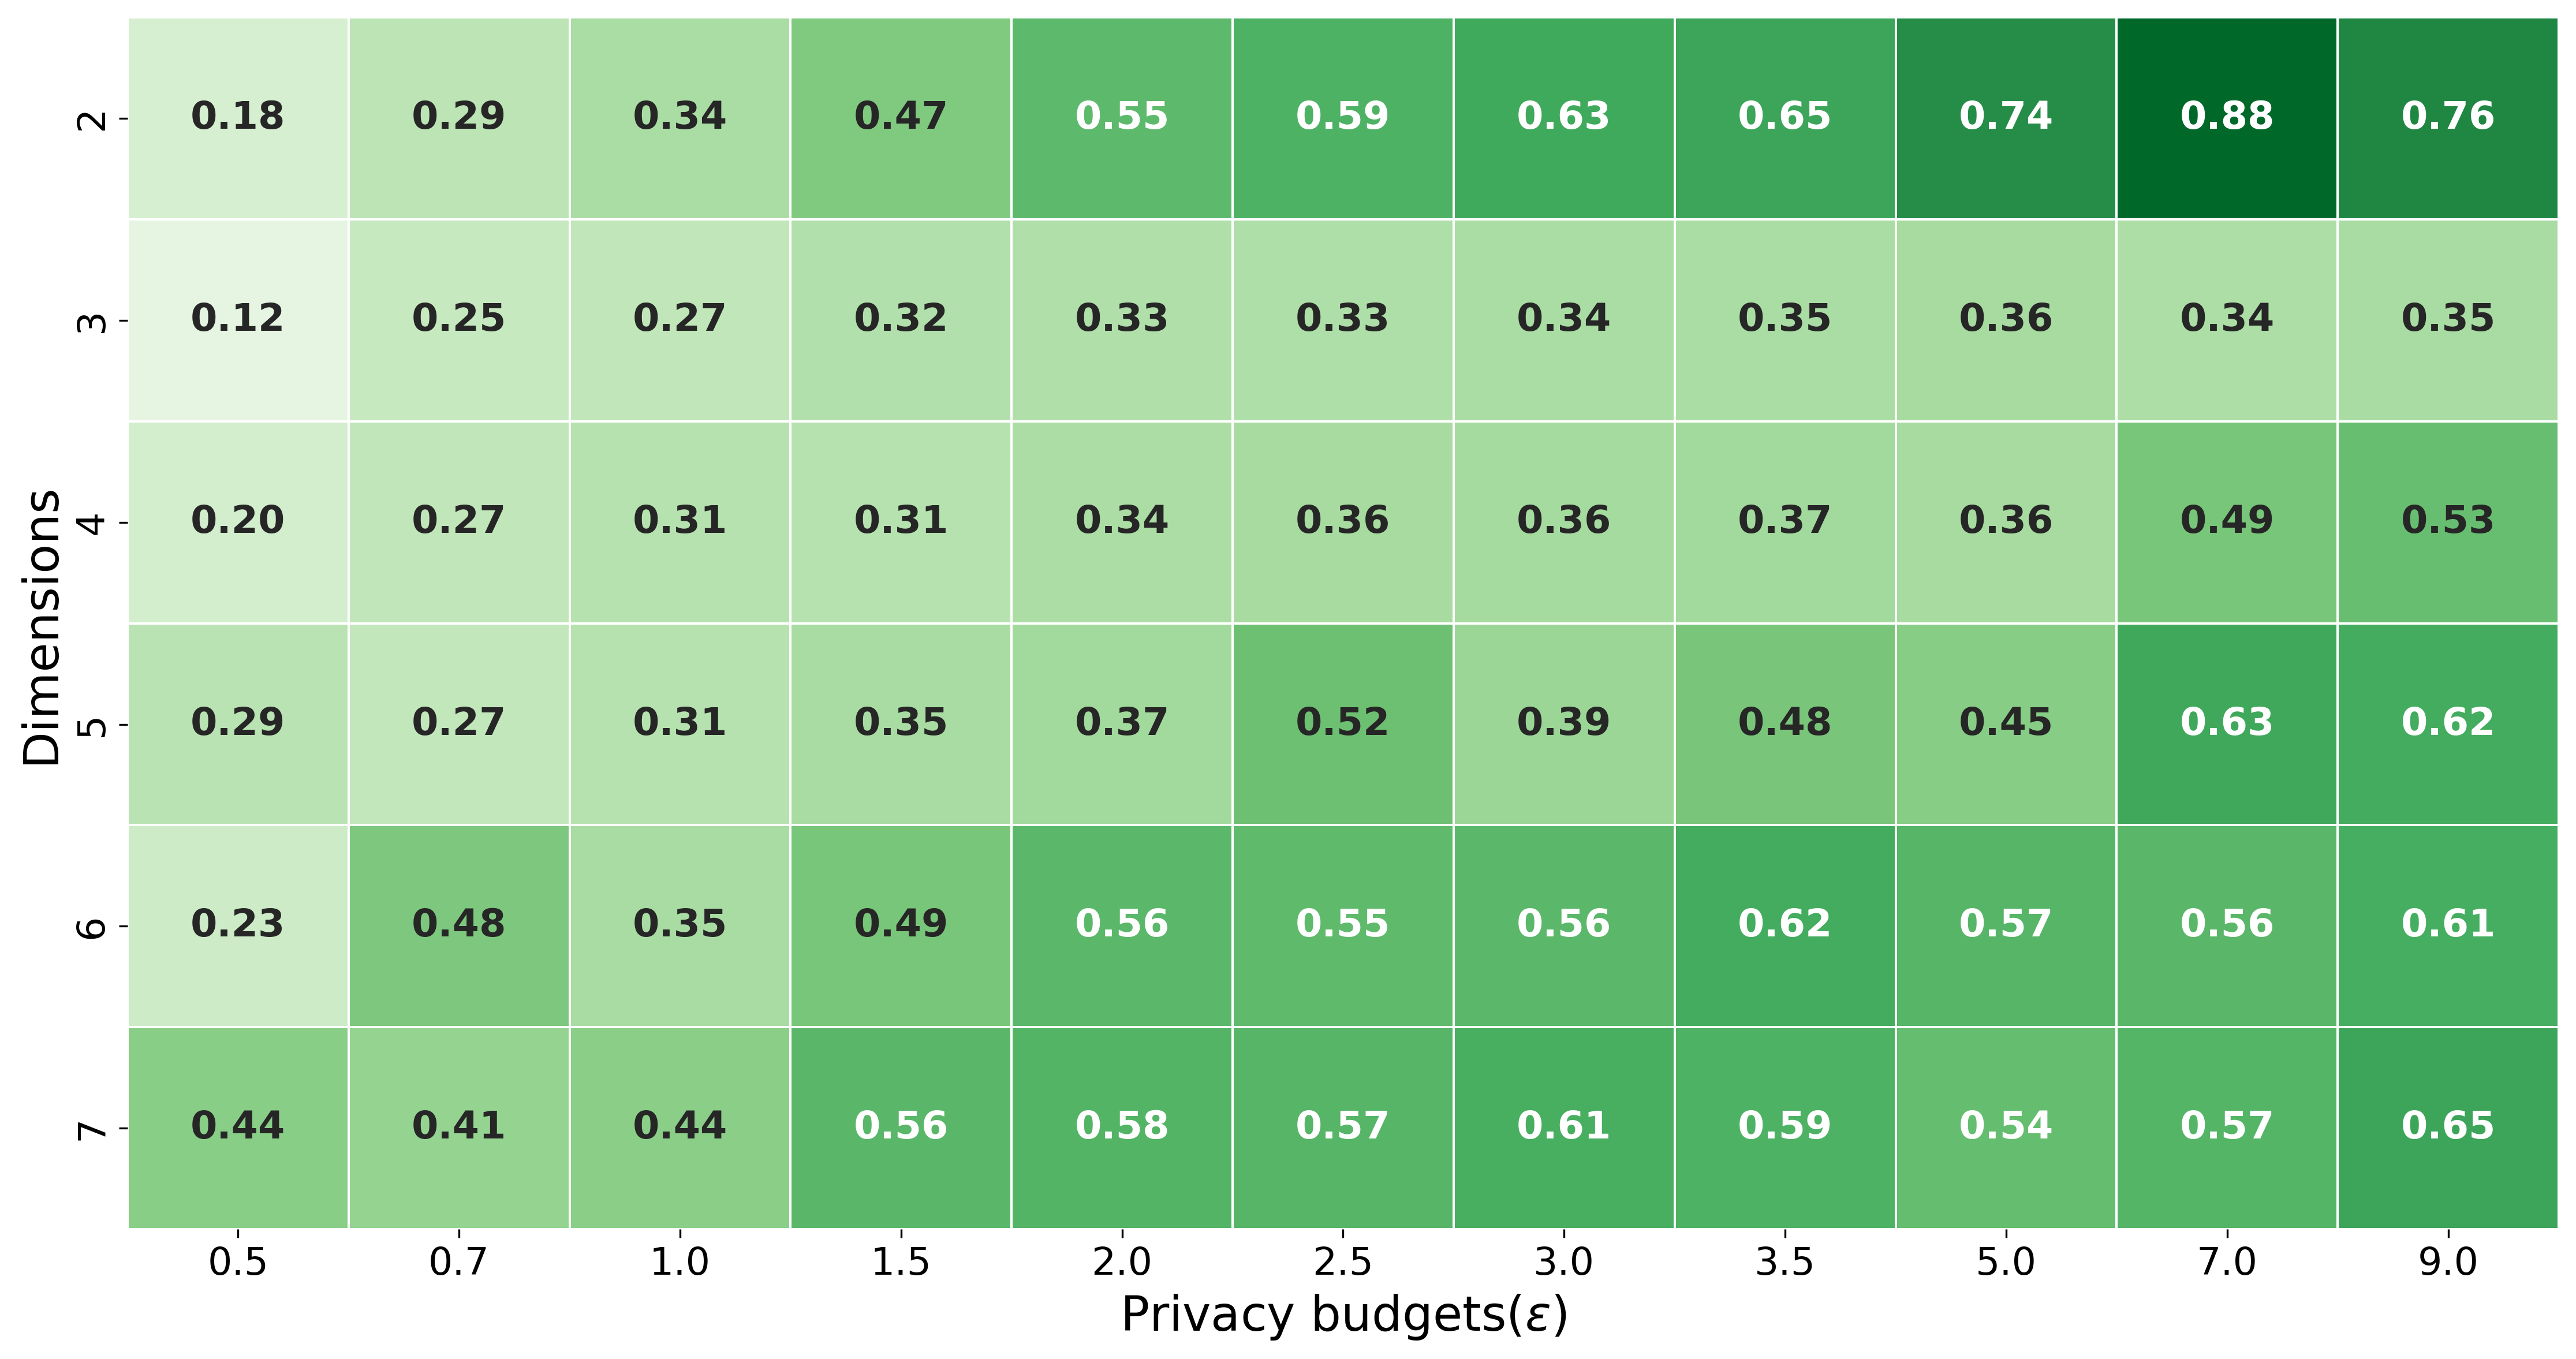
\includegraphics[width=1\textwidth]{Results/kd-laplace/grid-kd-Laplace/seeds-dataset/ami.png}
            \label{fig:ami_seeds-dataset_comparison_grid-kd_2d}
        \end{subfigure}
        \vfill % vertical space
        \begin{subfigure}[c]{1\textwidth}
            \caption{\textbf{Adjusted Mutual Information comparison for the density-kD-Laplace mechanism}}
            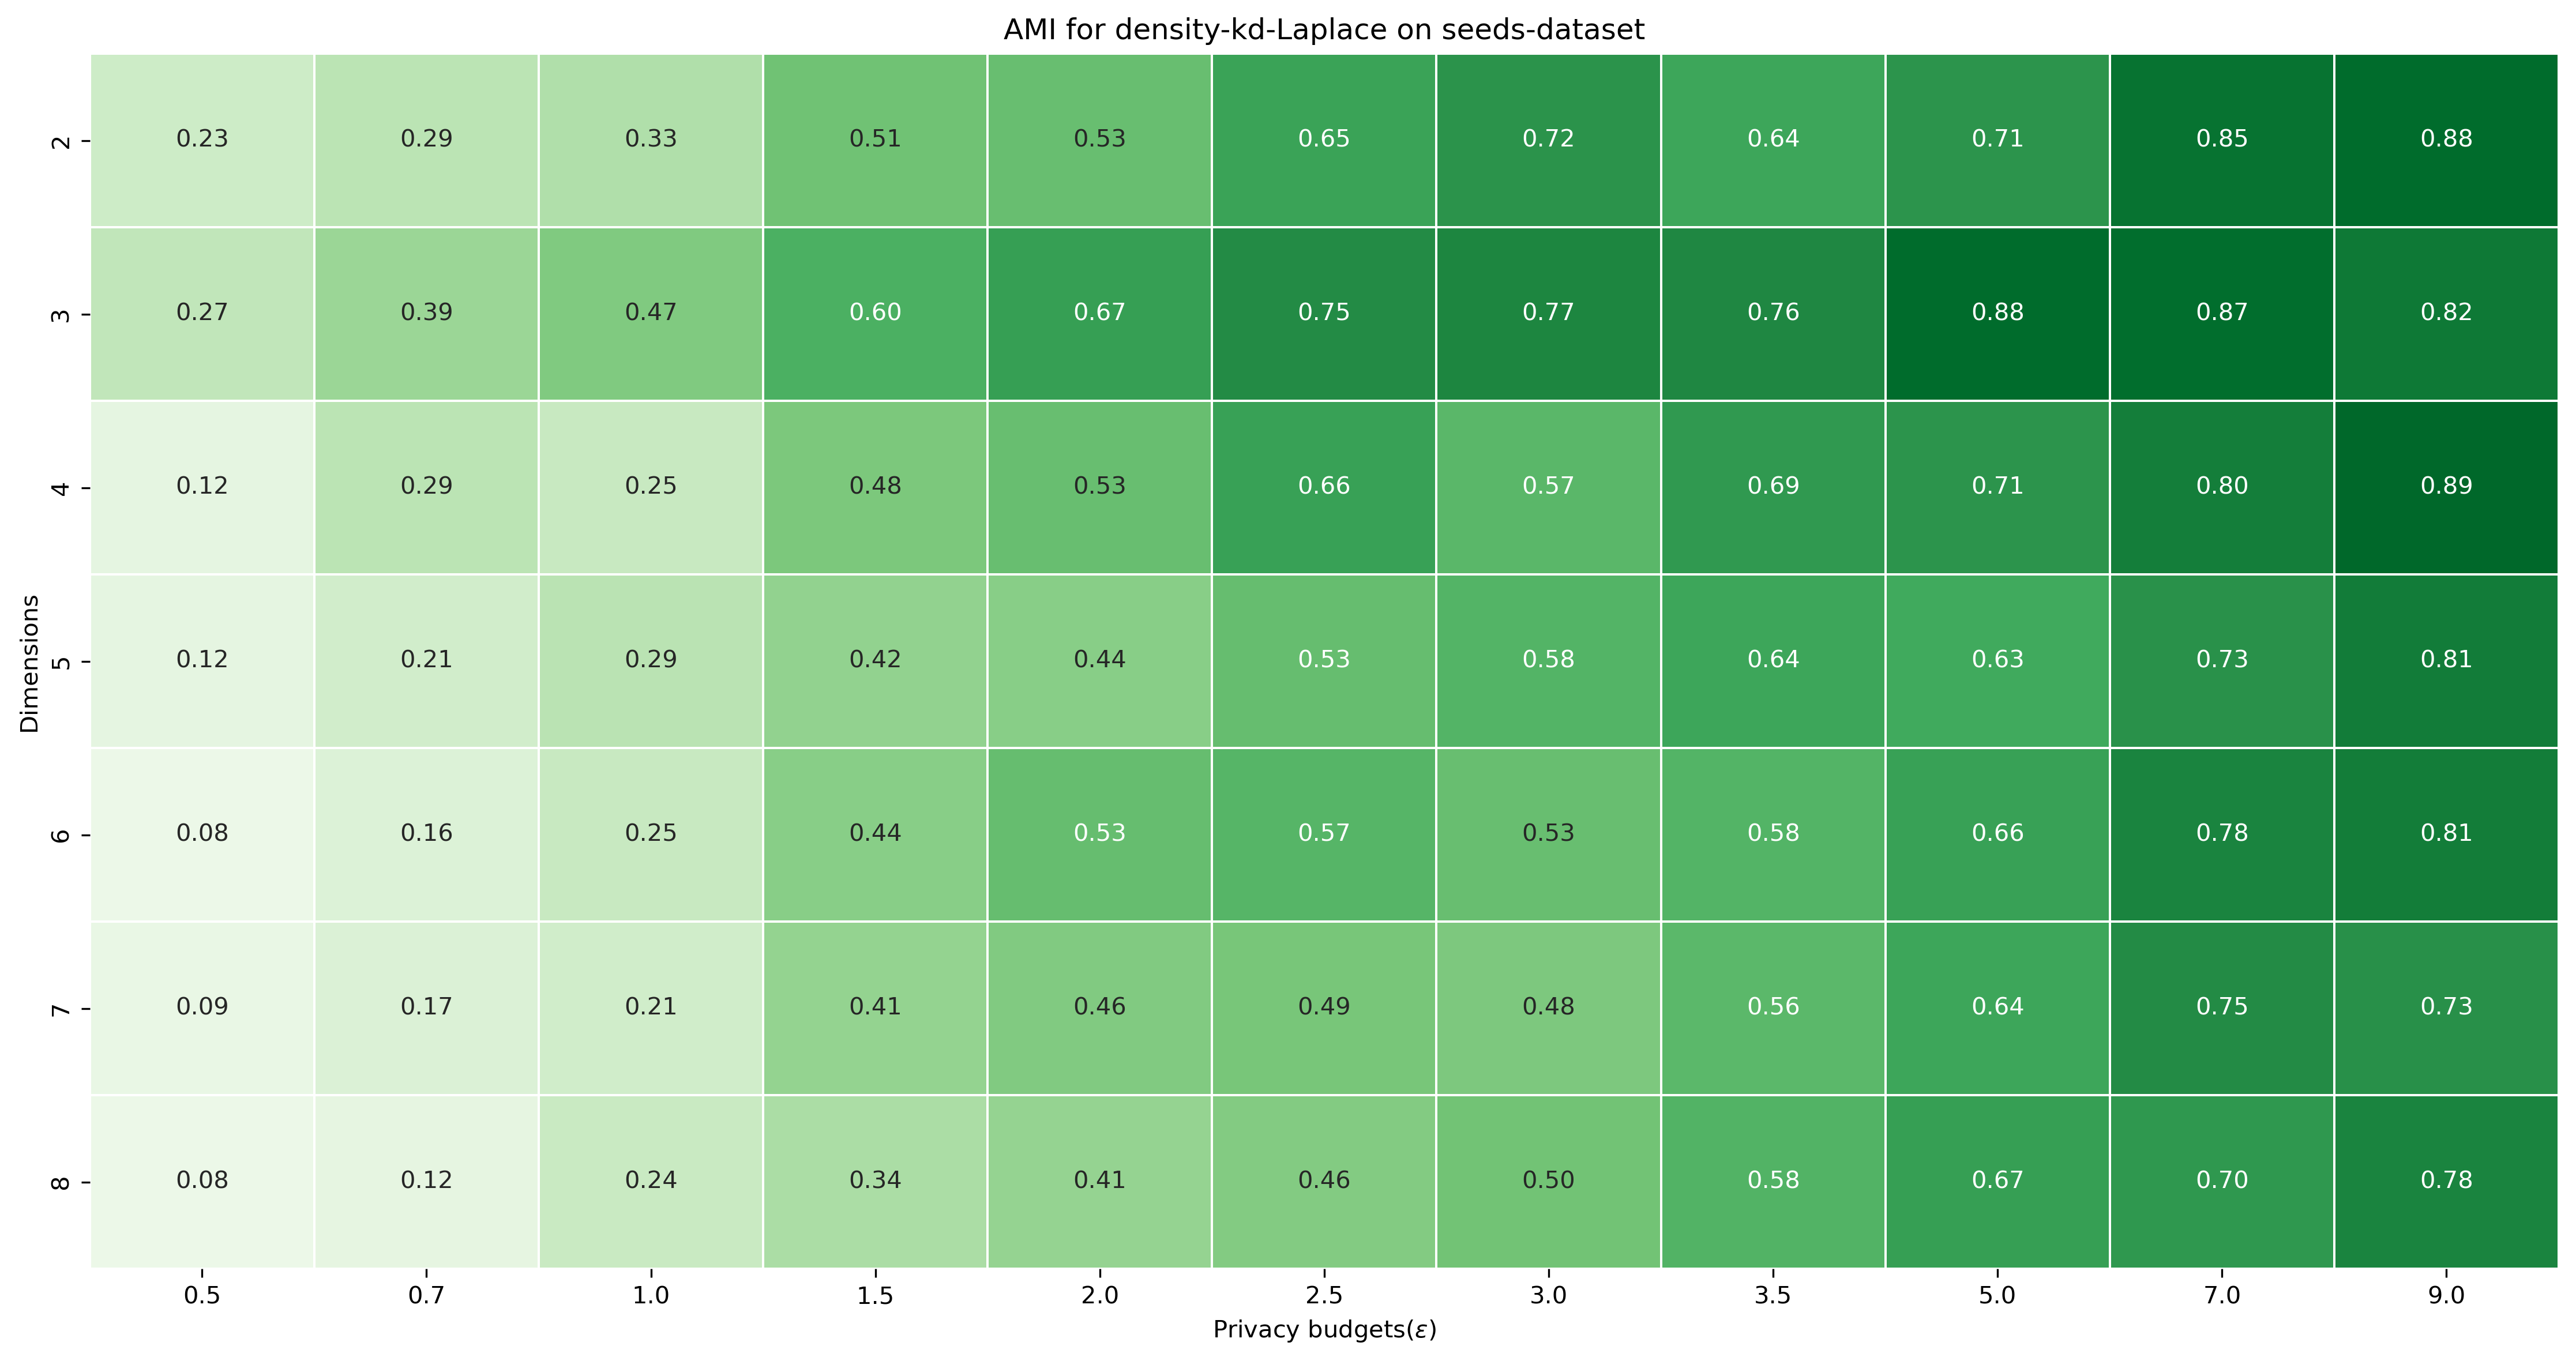
\includegraphics[width=1\textwidth]{Results/kd-laplace/density-kd-Laplace/seeds-dataset/ami.png}
            \label{fig:ami_seeds-dataset_comparison_density-kd_2d}
        \end{subfigure}
    \end{subfigure}
\end{figure}
\todo[inline]{Add comments}
\newpage
\subsection{Heart dataset} \label{appendix:results-mechanism-utility-heart-dataset}
\begin{figure}[H]
    \centering
    \begin{subfigure}[b]{0.90\textwidth}
        \begin{subfigure}[c]{1\textwidth}
            \caption{\textbf{Adjusted Mutual Information comparison for the grid-kD-Laplace mechanism}}
            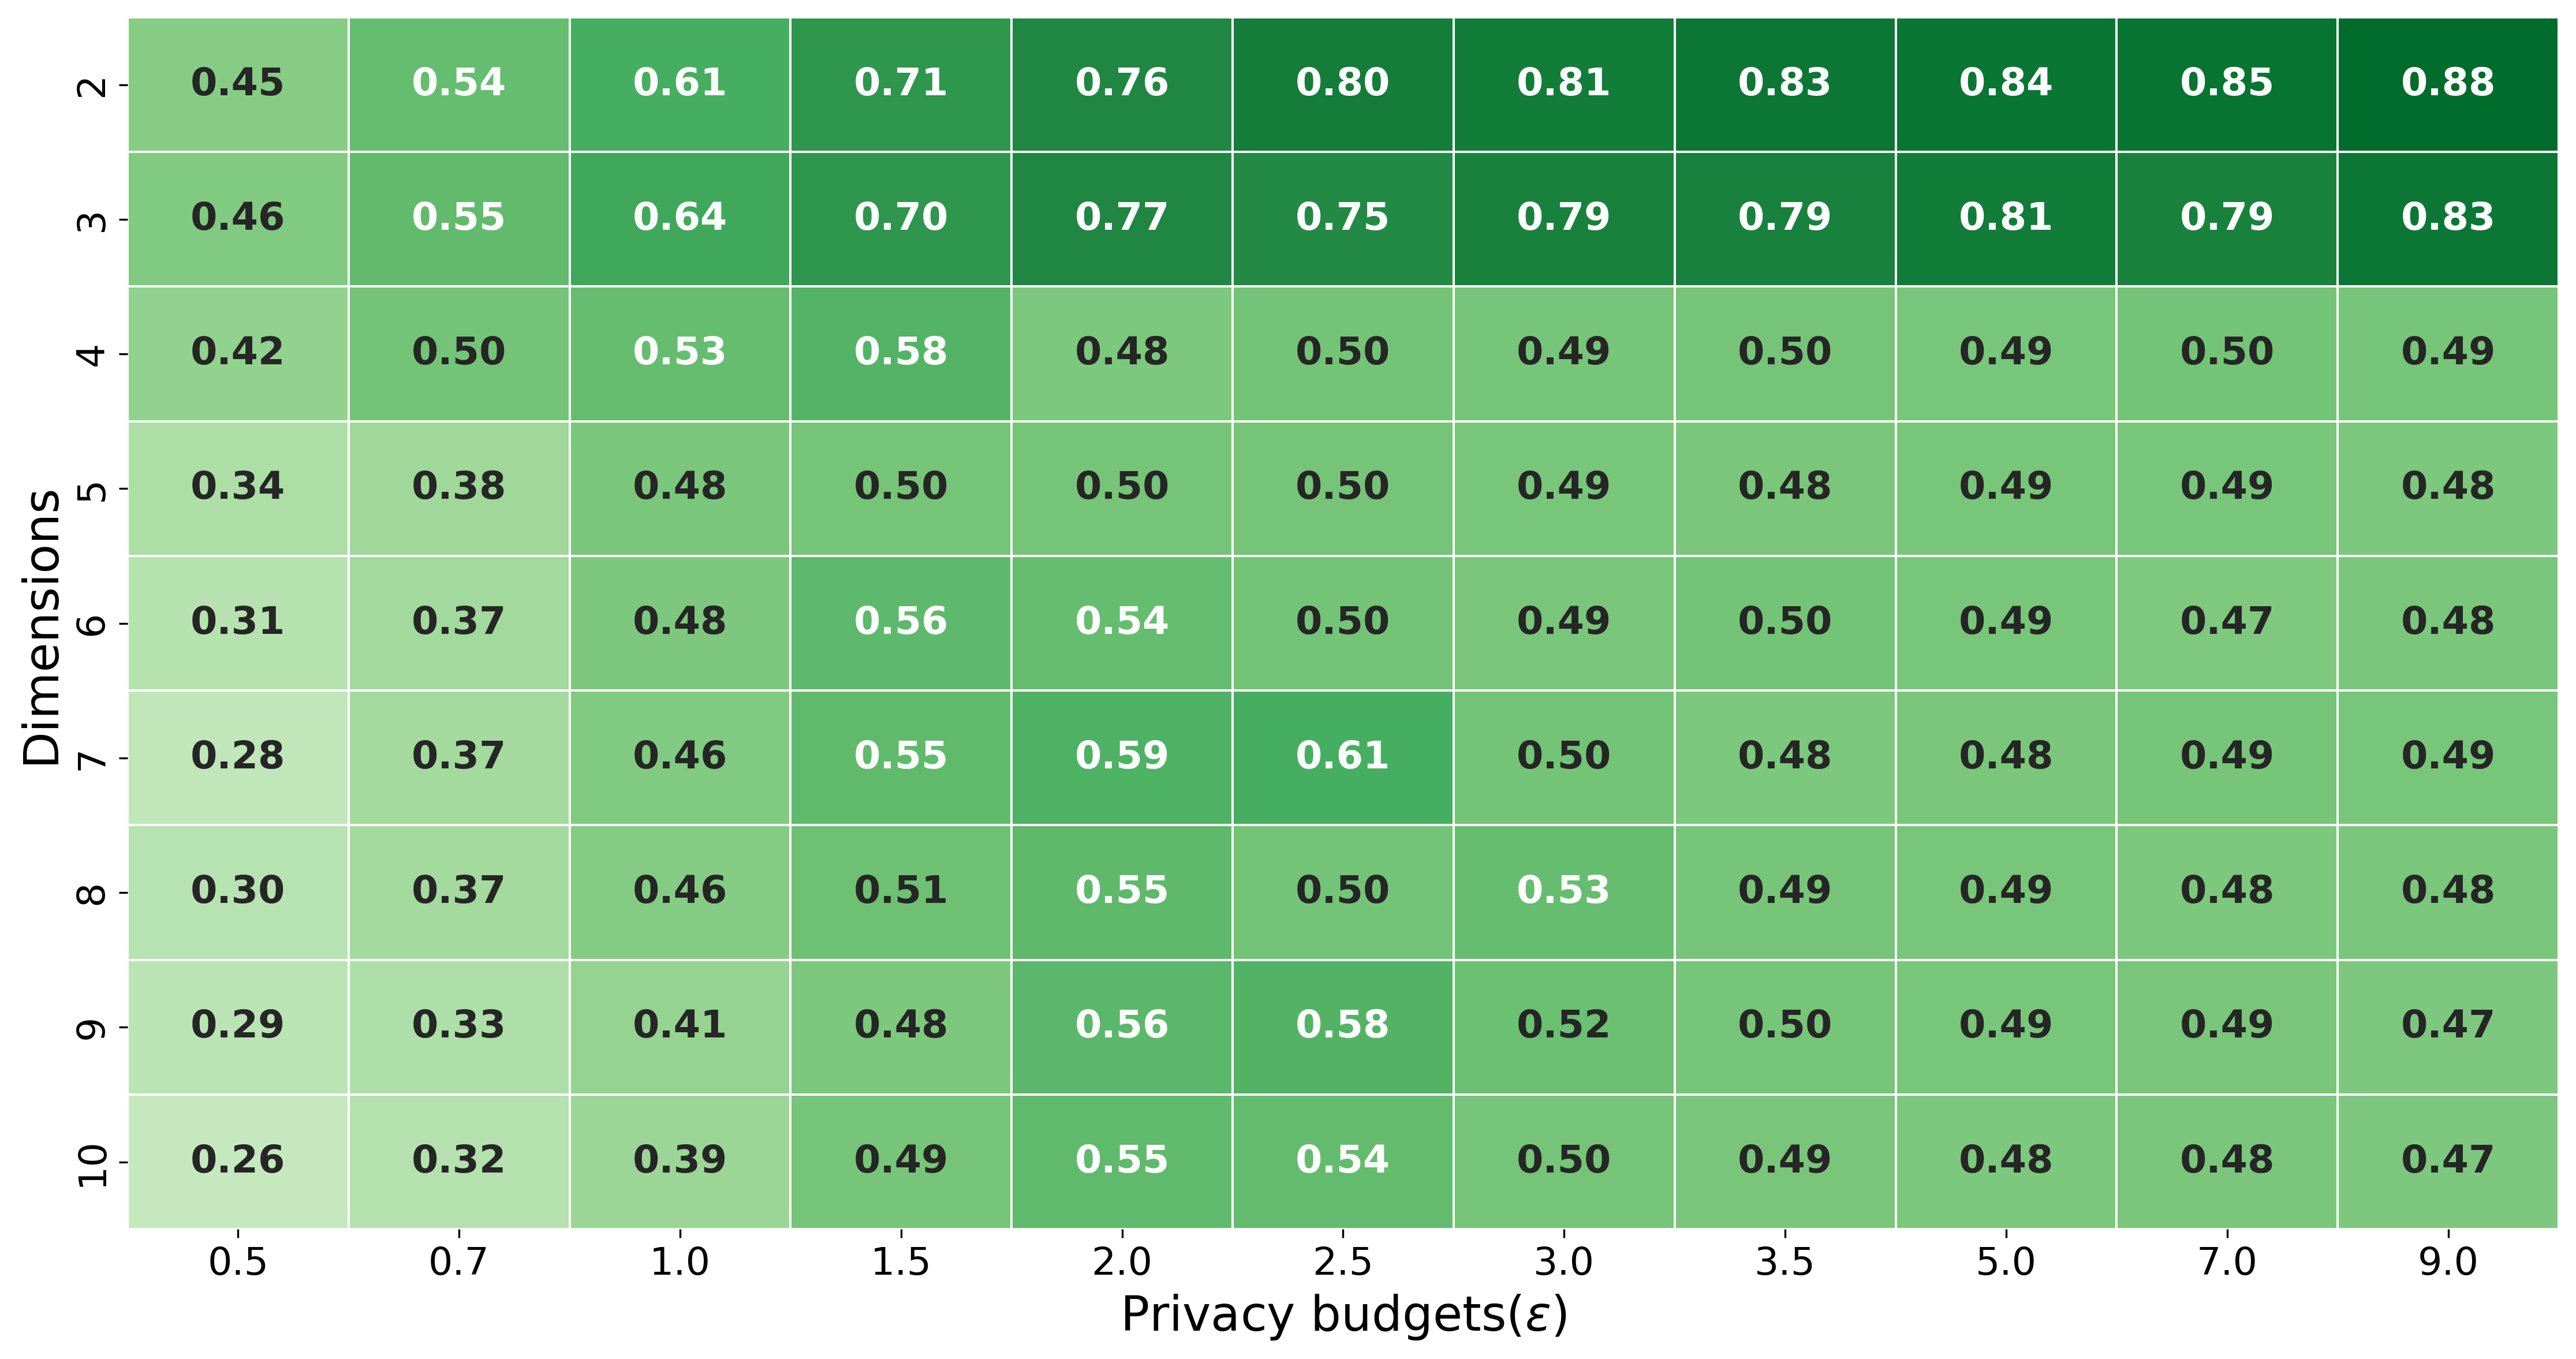
\includegraphics[width=1\textwidth]{Results/kd-laplace/grid-kd-Laplace/heart-dataset/ami.png}
            \label{fig:ami_heart-dataset_comparison_grid-kd_2d}
        \end{subfigure}
        \vfill % vertical space
        \begin{subfigure}[c]{1\textwidth}
            \caption{\textbf{Adjusted Mutual Information comparison for the density-kD-Laplace mechanism}}
            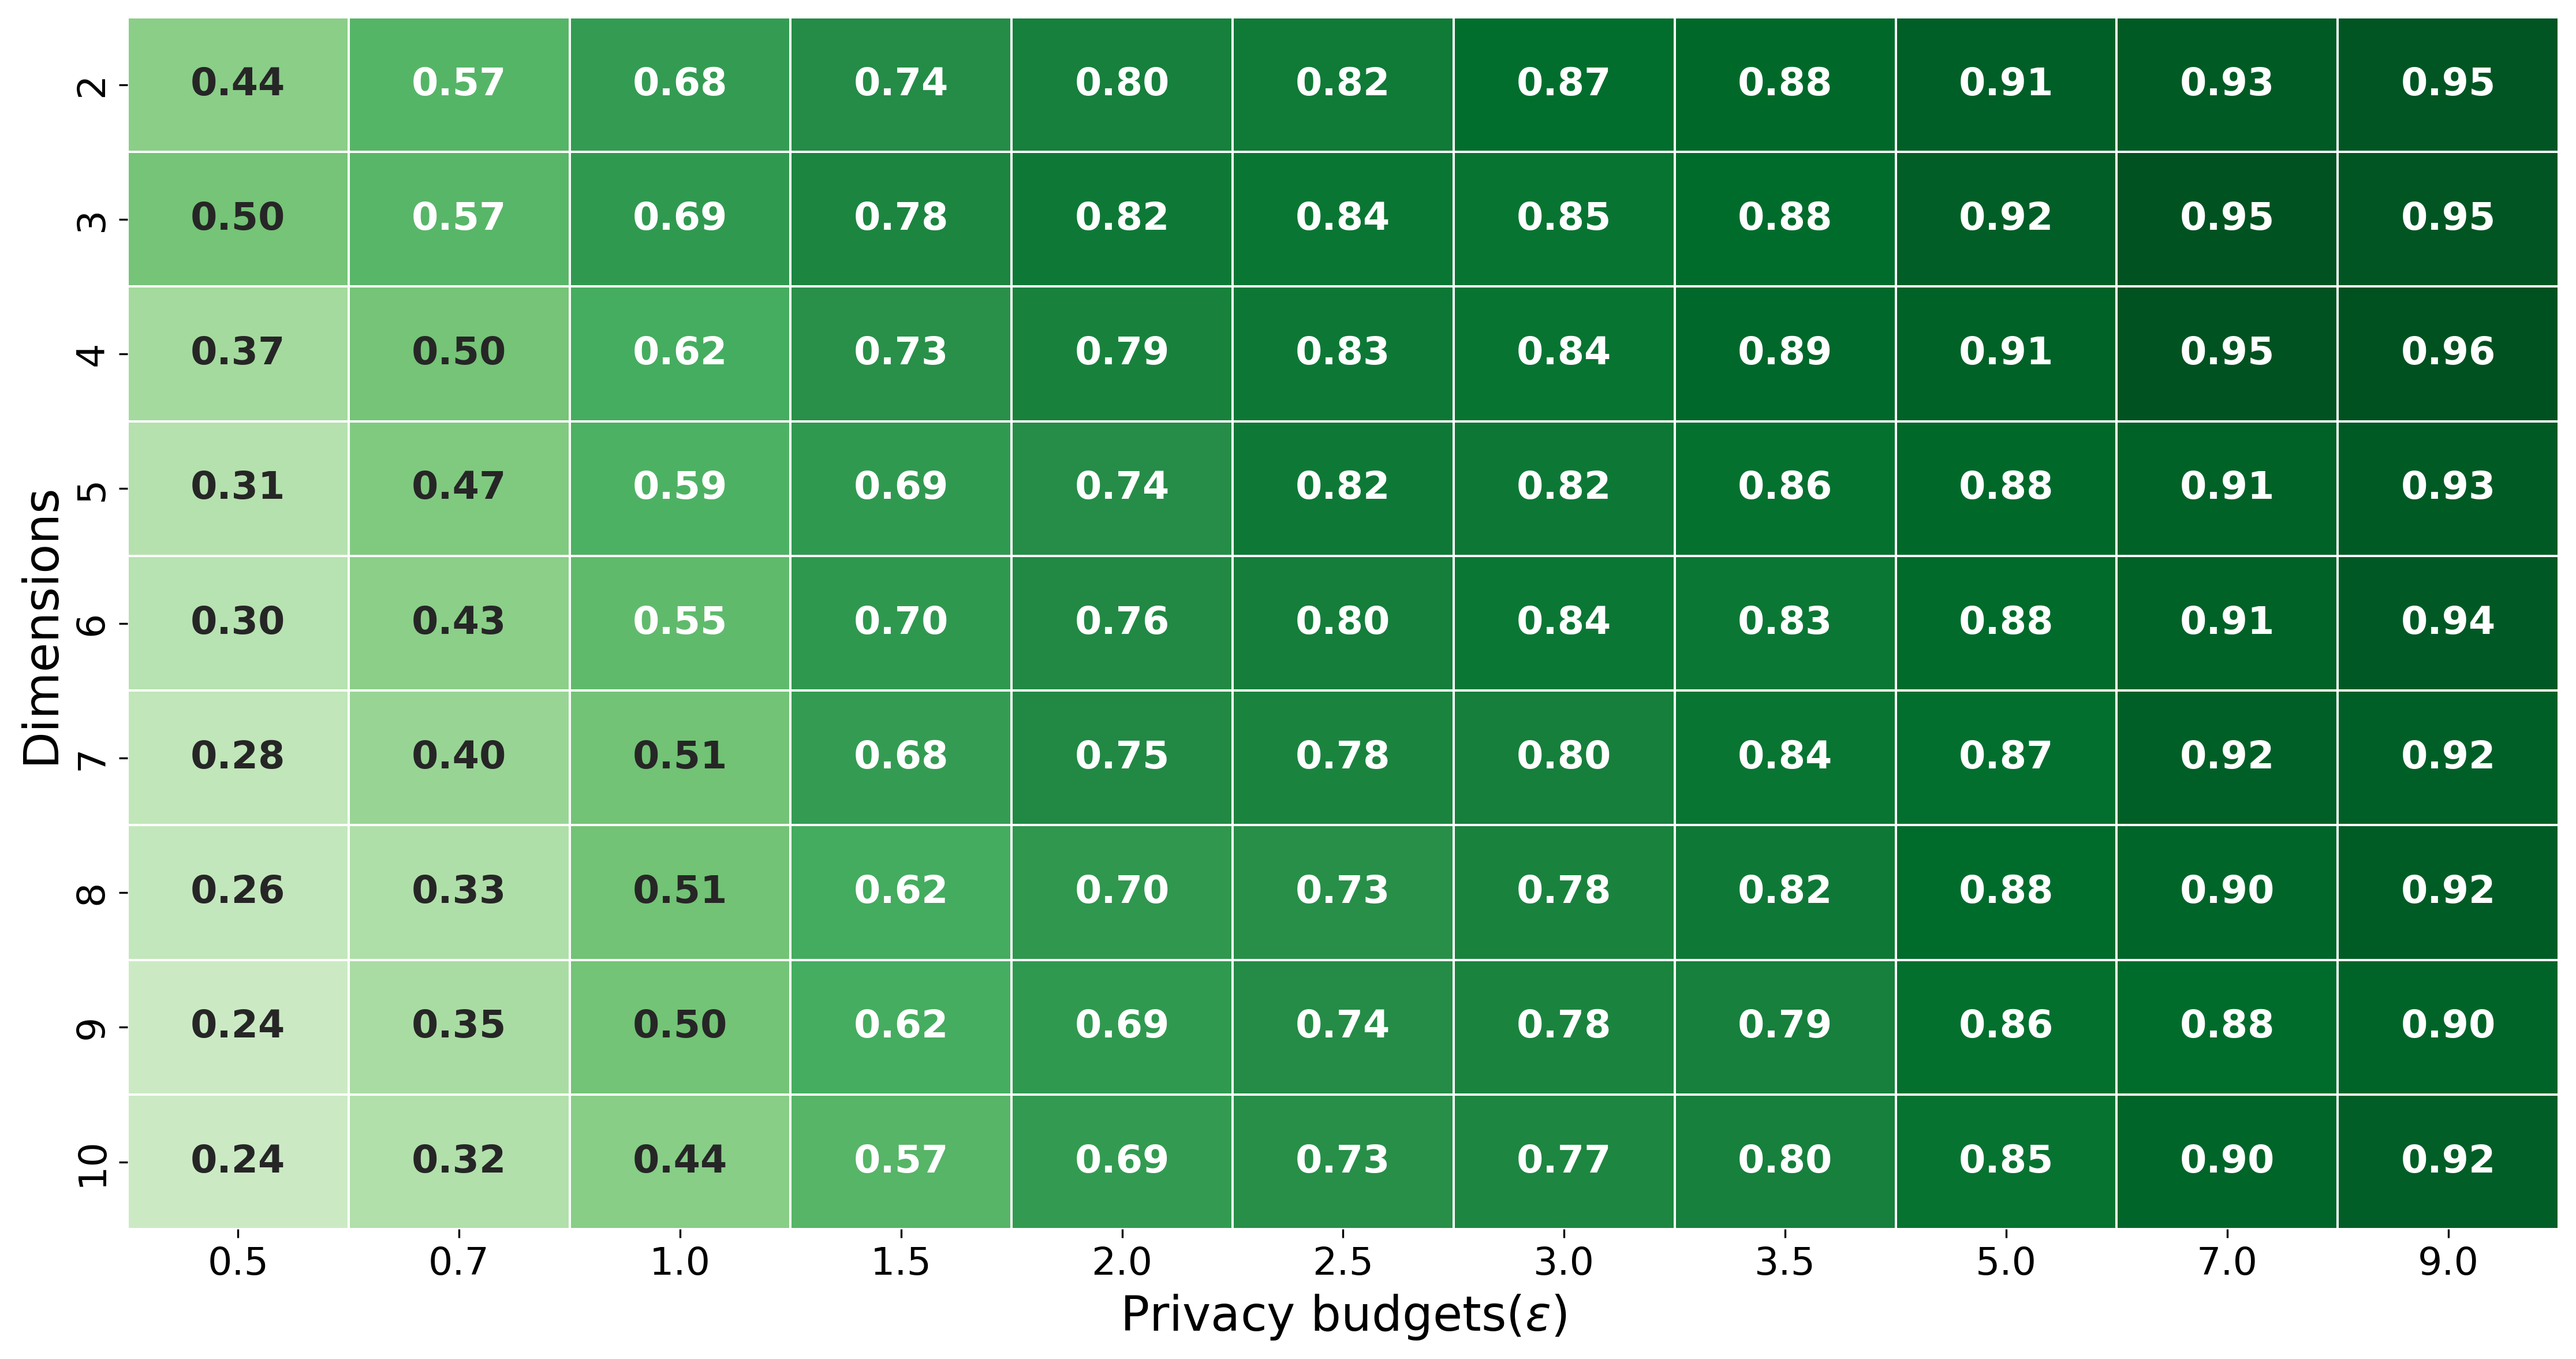
\includegraphics[width=1\textwidth]{Results/kd-laplace/density-kd-Laplace/heart-dataset/ami.png}
            \label{fig:ami_heart-dataset_comparison_density-kd_2d}
        \end{subfigure}
    \end{subfigure}
\end{figure}
\todo[inline]{Add comments}
\newpage
\subsection{Circle dataset} \label{appendix:results-mechanism-utility-circle-dataset}
\begin{figure}[H]
    \centering
    \begin{subfigure}[b]{0.90\textwidth}
        \begin{subfigure}[c]{1\textwidth}
            \caption{\textbf{Adjusted Mutual Information comparison for the grid-kD-Laplace mechanism}}
            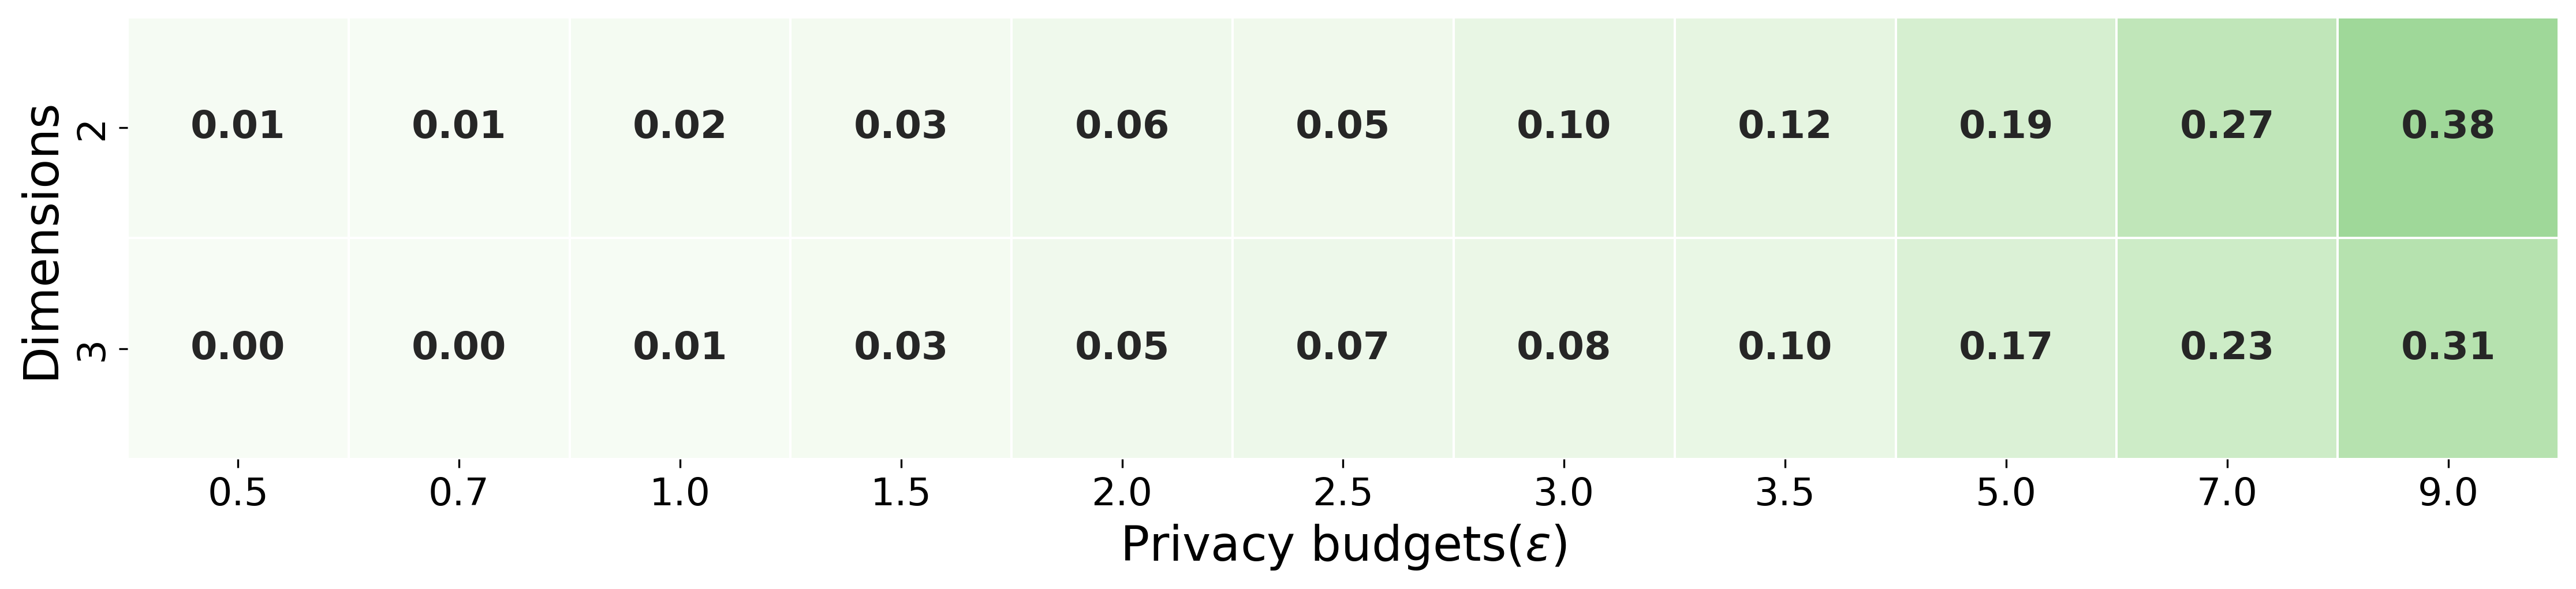
\includegraphics[width=1\textwidth]{Results/kd-laplace/grid-kd-Laplace/circle-dataset/ami.png}
            \label{fig:ami_circle-dataset_comparison_grid-kd_2d}
        \end{subfigure}
        \vfill % vertical space
        \begin{subfigure}[c]{1\textwidth}
            \caption{\textbf{Adjusted Mutual Information comparison for the density-kD-Laplace mechanism}}
            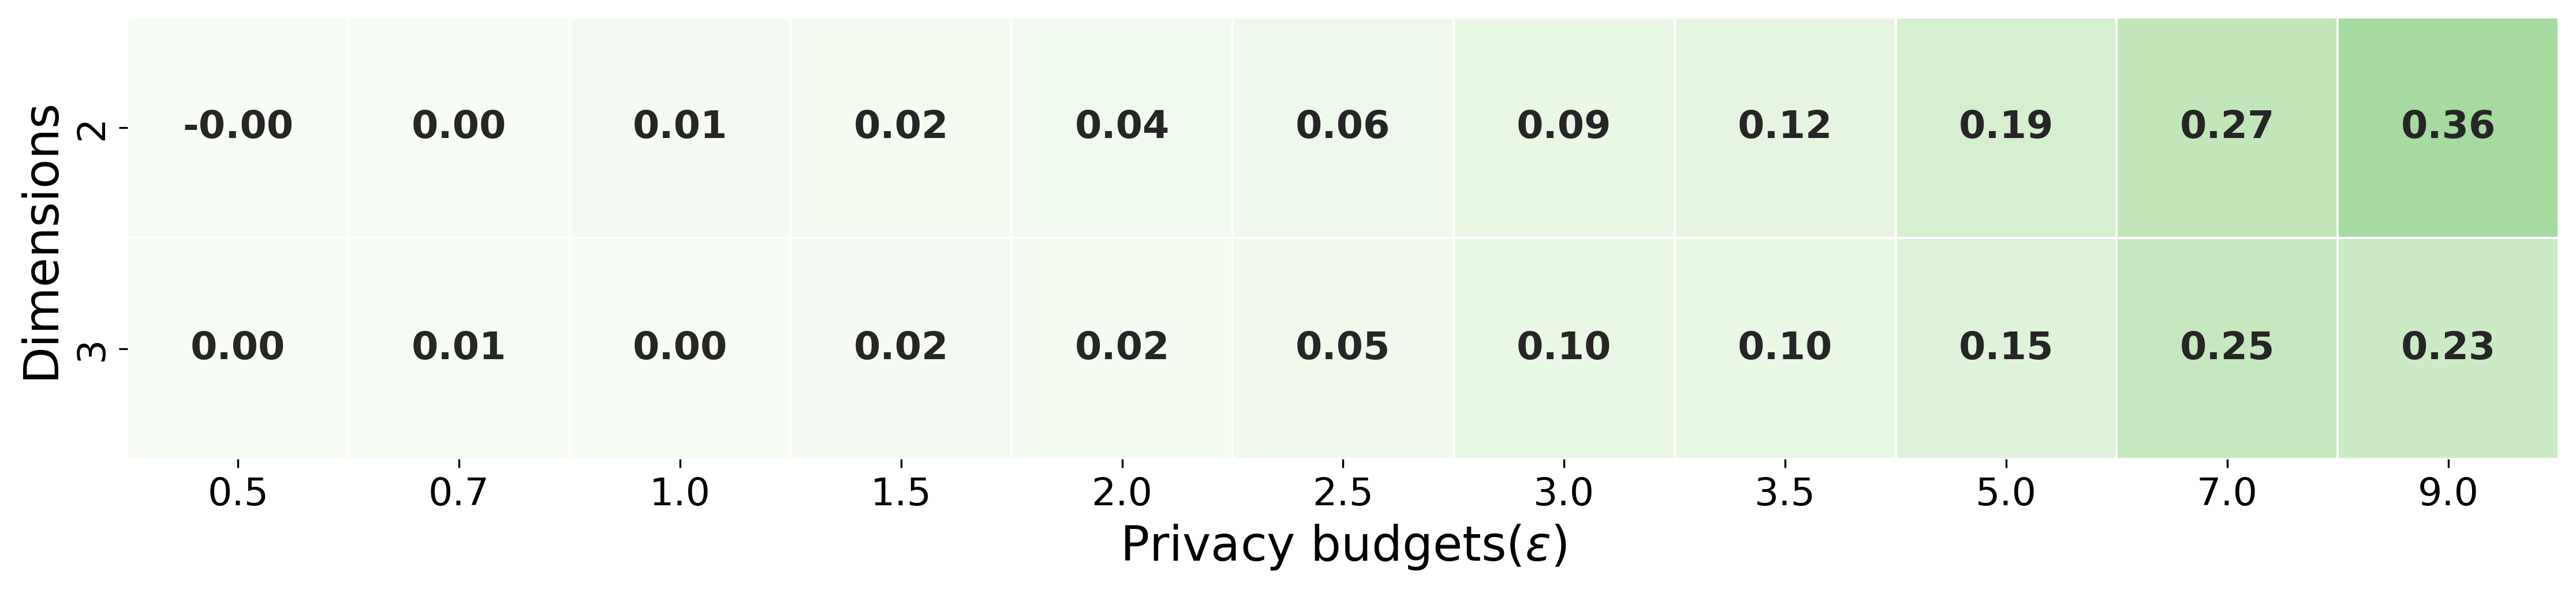
\includegraphics[width=1\textwidth]{Results/kd-laplace/density-kd-Laplace/circle-dataset/ami.png}
            \label{fig:ami_circle-dataset_comparison_density-kd_2d}
        \end{subfigure}
    \end{subfigure}
\end{figure}
\todo[inline]{Add comments}
\newpage
\subsection{Line dataset} \label{appendix:results-mechanism-utility-line-dataset}
\begin{figure}[H]
    \centering
    \begin{subfigure}[b]{0.90\textwidth}
        \begin{subfigure}[c]{1\textwidth}
            \caption{\textbf{Adjusted Mutual Information comparison for the grid-kD-Laplace mechanism}}
            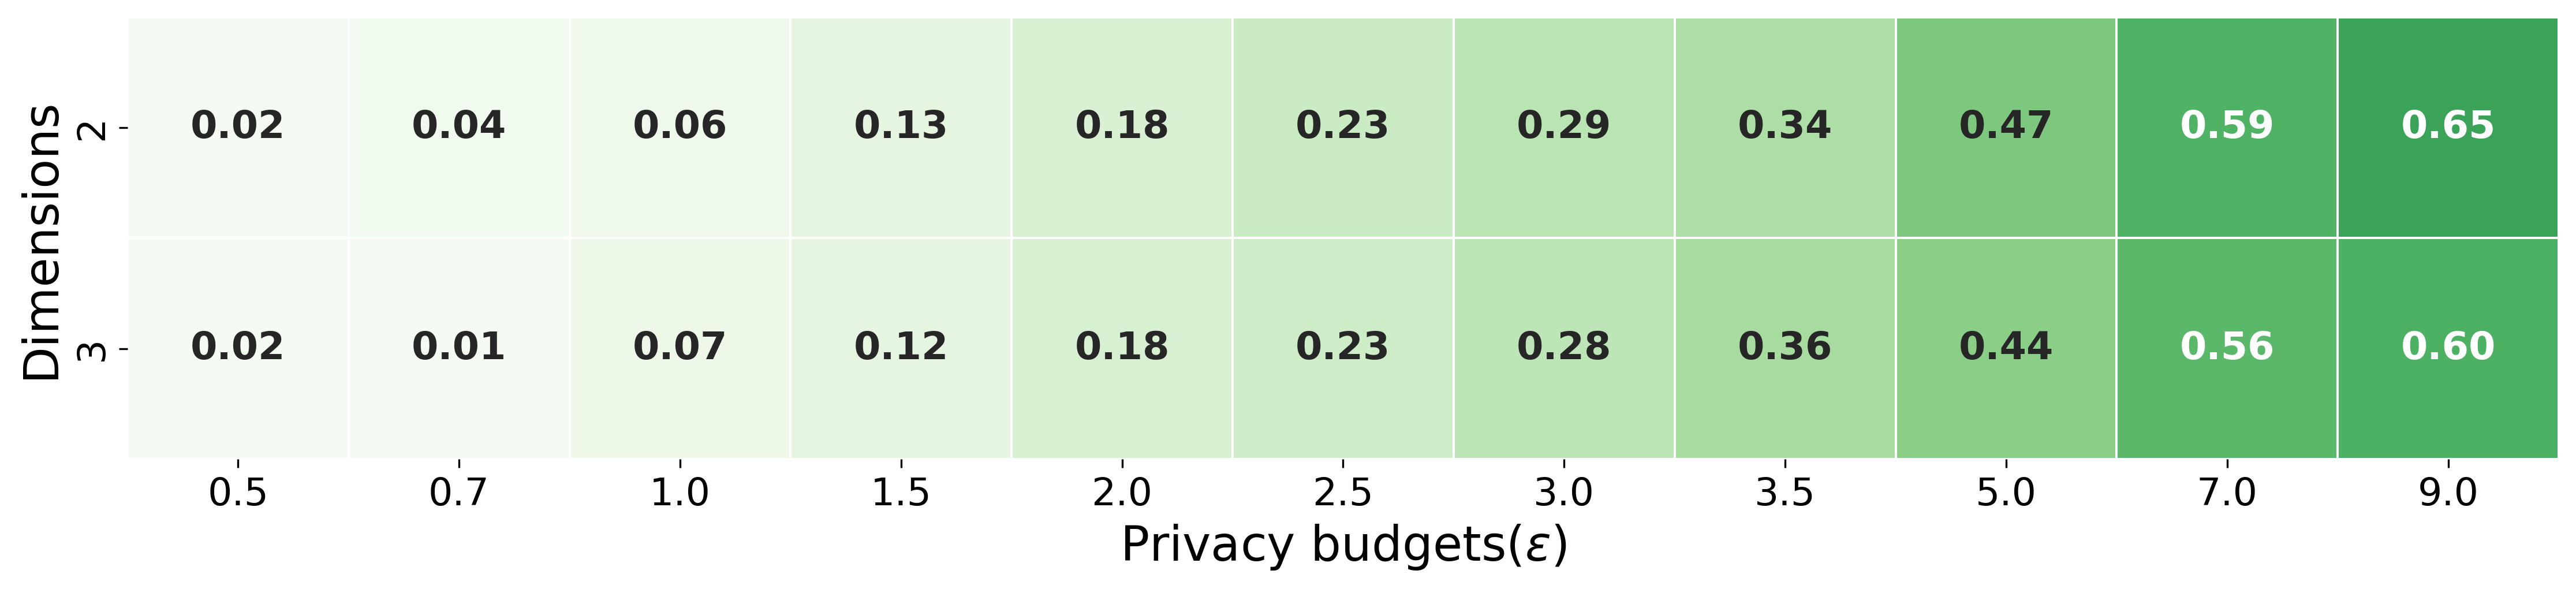
\includegraphics[width=1\textwidth]{Results/kd-laplace/grid-kd-Laplace/line-dataset/ami.png}
            \label{fig:ami_line-dataset_comparison_grid-kd_2d}
        \end{subfigure}
        \vfill % vertical space
        \begin{subfigure}[c]{1\textwidth}
            \caption{\textbf{Adjusted Mutual Information comparison for the density-kD-Laplace mechanism}}
            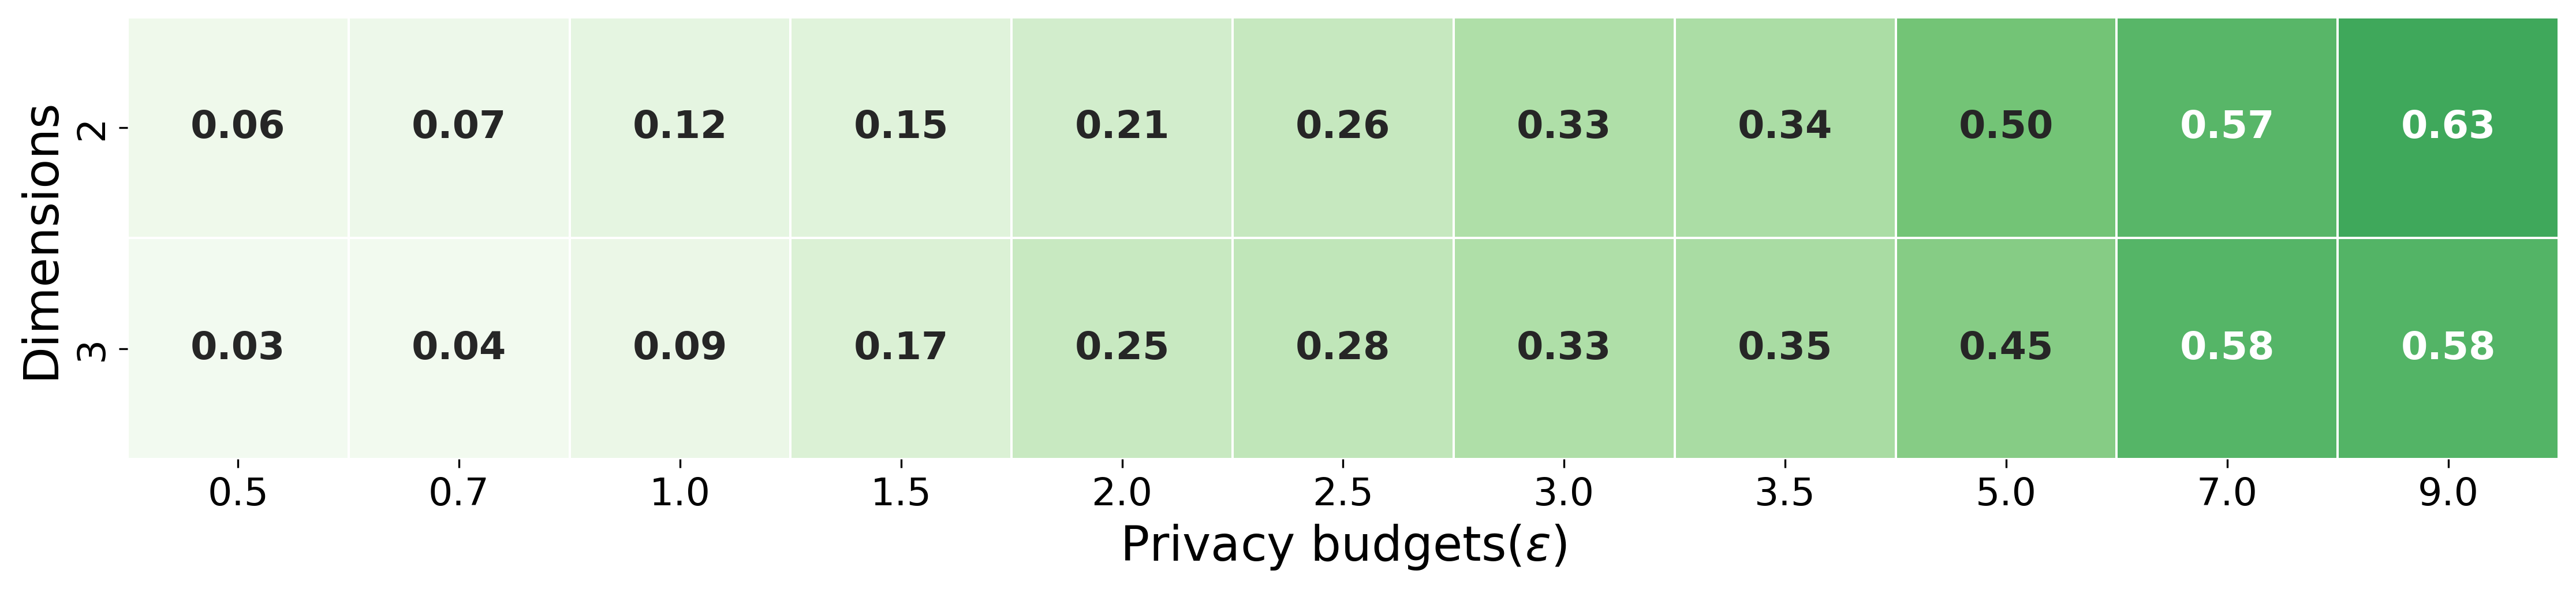
\includegraphics[width=1\textwidth]{Results/kd-laplace/density-kd-Laplace/line-dataset/ami.png}
            \label{fig:ami_line-dataset_comparison_density-kd_2d}
        \end{subfigure}
    \end{subfigure}
\end{figure}
\todo[inline]{Add comments}
\newpage
\subsection{Skewed dataset} \label{appendix:results-mechanism-utility-skewed-dataset}

\begin{figure}[H]
    \centering
    \begin{subfigure}[b]{0.90\textwidth}
        \begin{subfigure}[c]{1\textwidth}
            \caption{\textbf{Adjusted Mutual Information comparison for the grid-kD-Laplace mechanism}}
            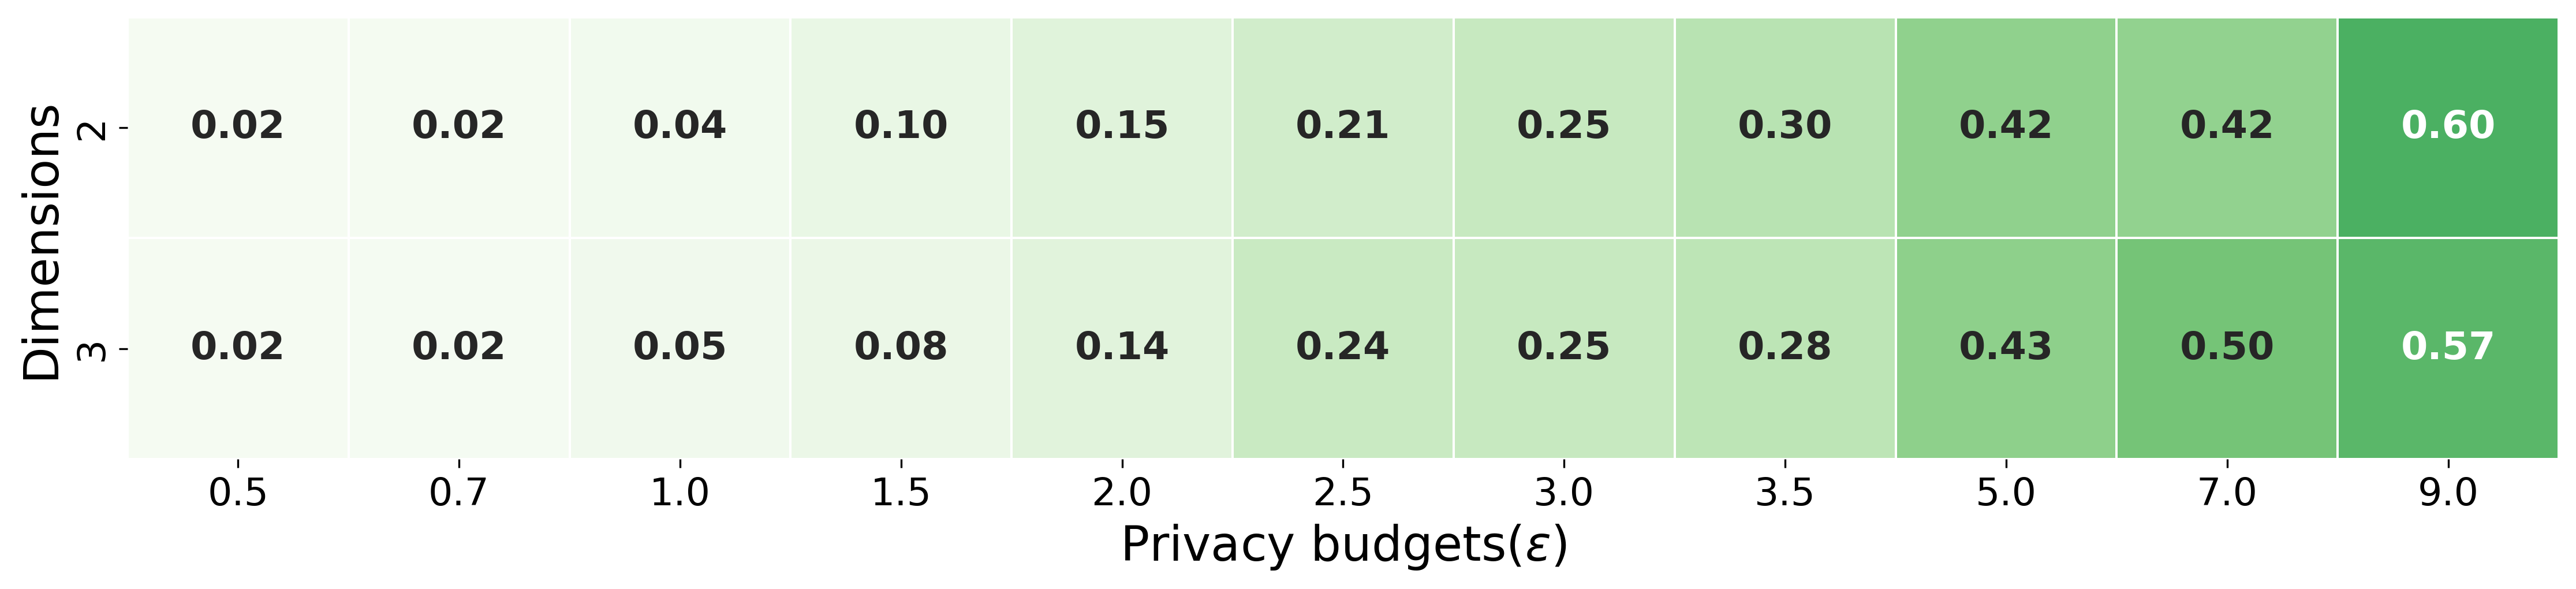
\includegraphics[width=1\textwidth]{Results/kd-laplace/grid-kd-Laplace/skewed-dataset/ami.png}
            \label{fig:ami_skewed-dataset_comparison_grid-kd_2d}
        \end{subfigure}
        \vfill % vertical space
        \begin{subfigure}[c]{1\textwidth}
            \caption{\textbf{Adjusted Mutual Information comparison for the density-kD-Laplace mechanism}}
            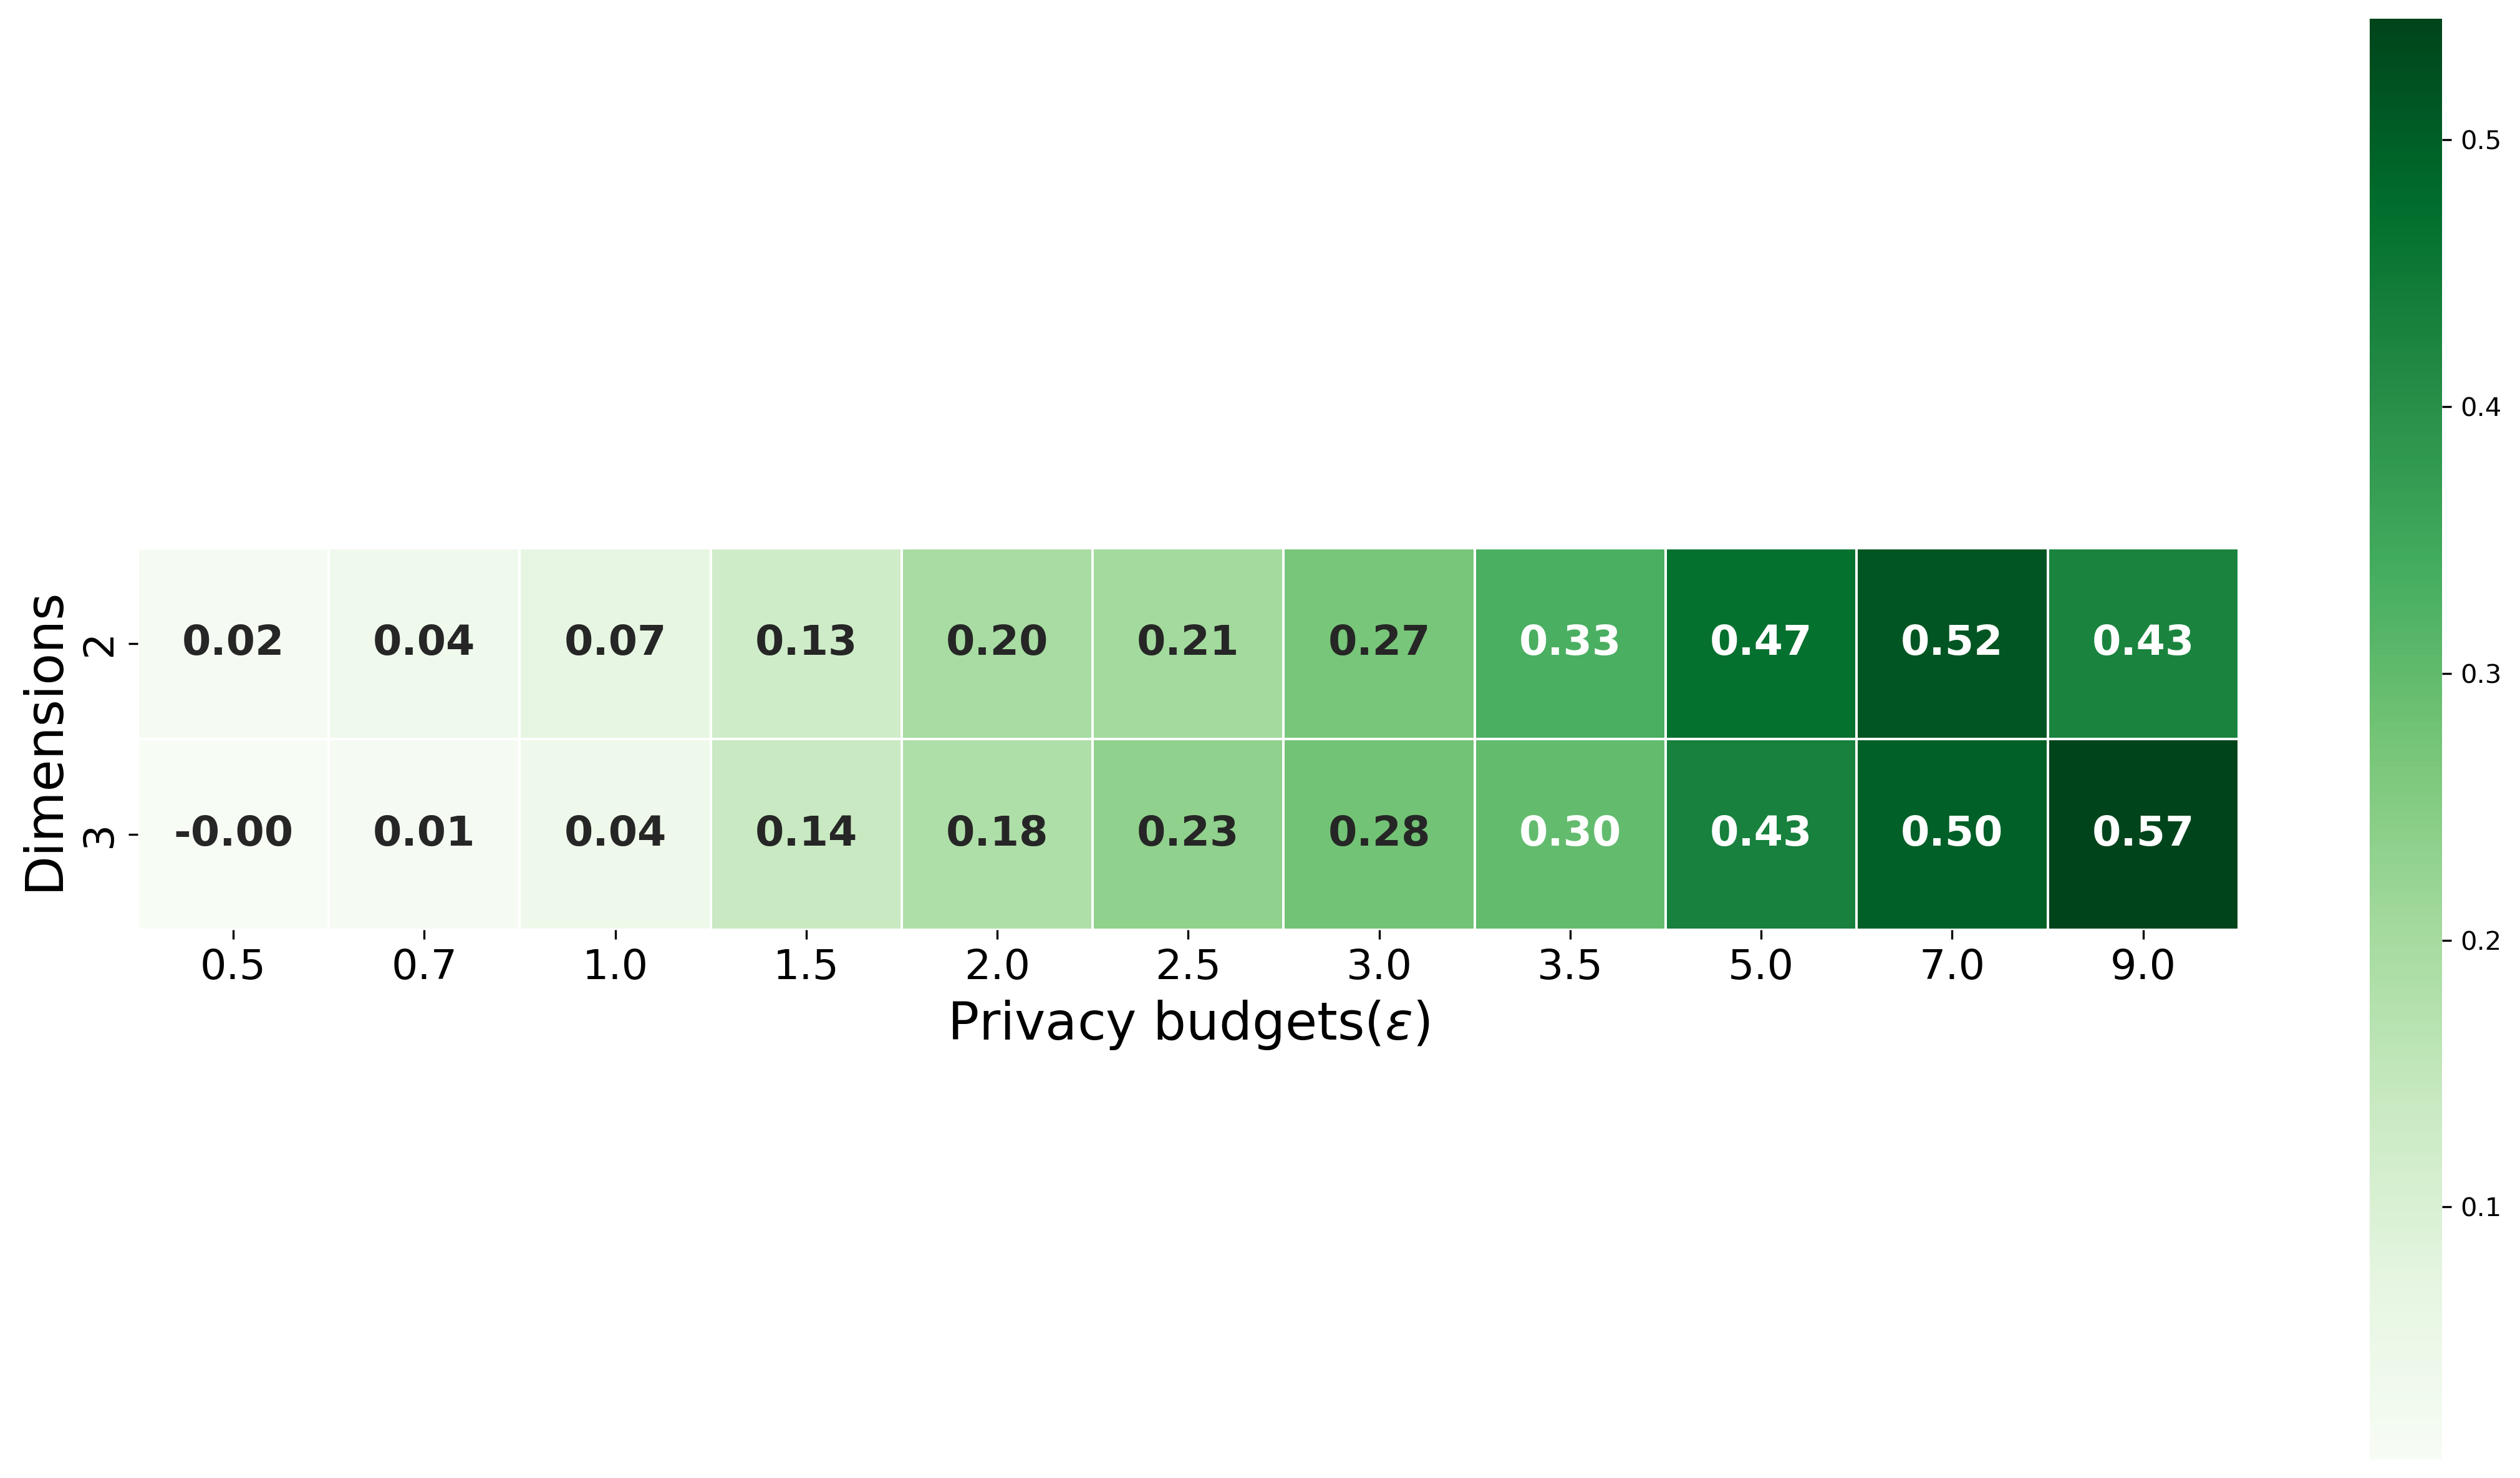
\includegraphics[width=1\textwidth]{Results/kd-laplace/density-kd-Laplace/skewed-dataset/ami.png}
            \label{fig:ami_skewed-dataset_comparison_density-kd_2d}
        \end{subfigure}
    \end{subfigure}
\end{figure}
\todo[inline]{Add comments}
\newpage
\section{Privacy} \label{appendix:results-privacy}
\subsection{Seeds dataset} \label{appendix:results-privacy-seeds-dataset}
\begin{figure}[H]
    \centering
    \begin{subfigure}[b]{0.9\textwidth}
        \begin{subfigure}[c]{1\textwidth}
            \caption{\textbf{Heatmap showing disclosure risk for the kD-Laplace mechanism, per privacy budget \& dimension for seeds-dataset.}}
            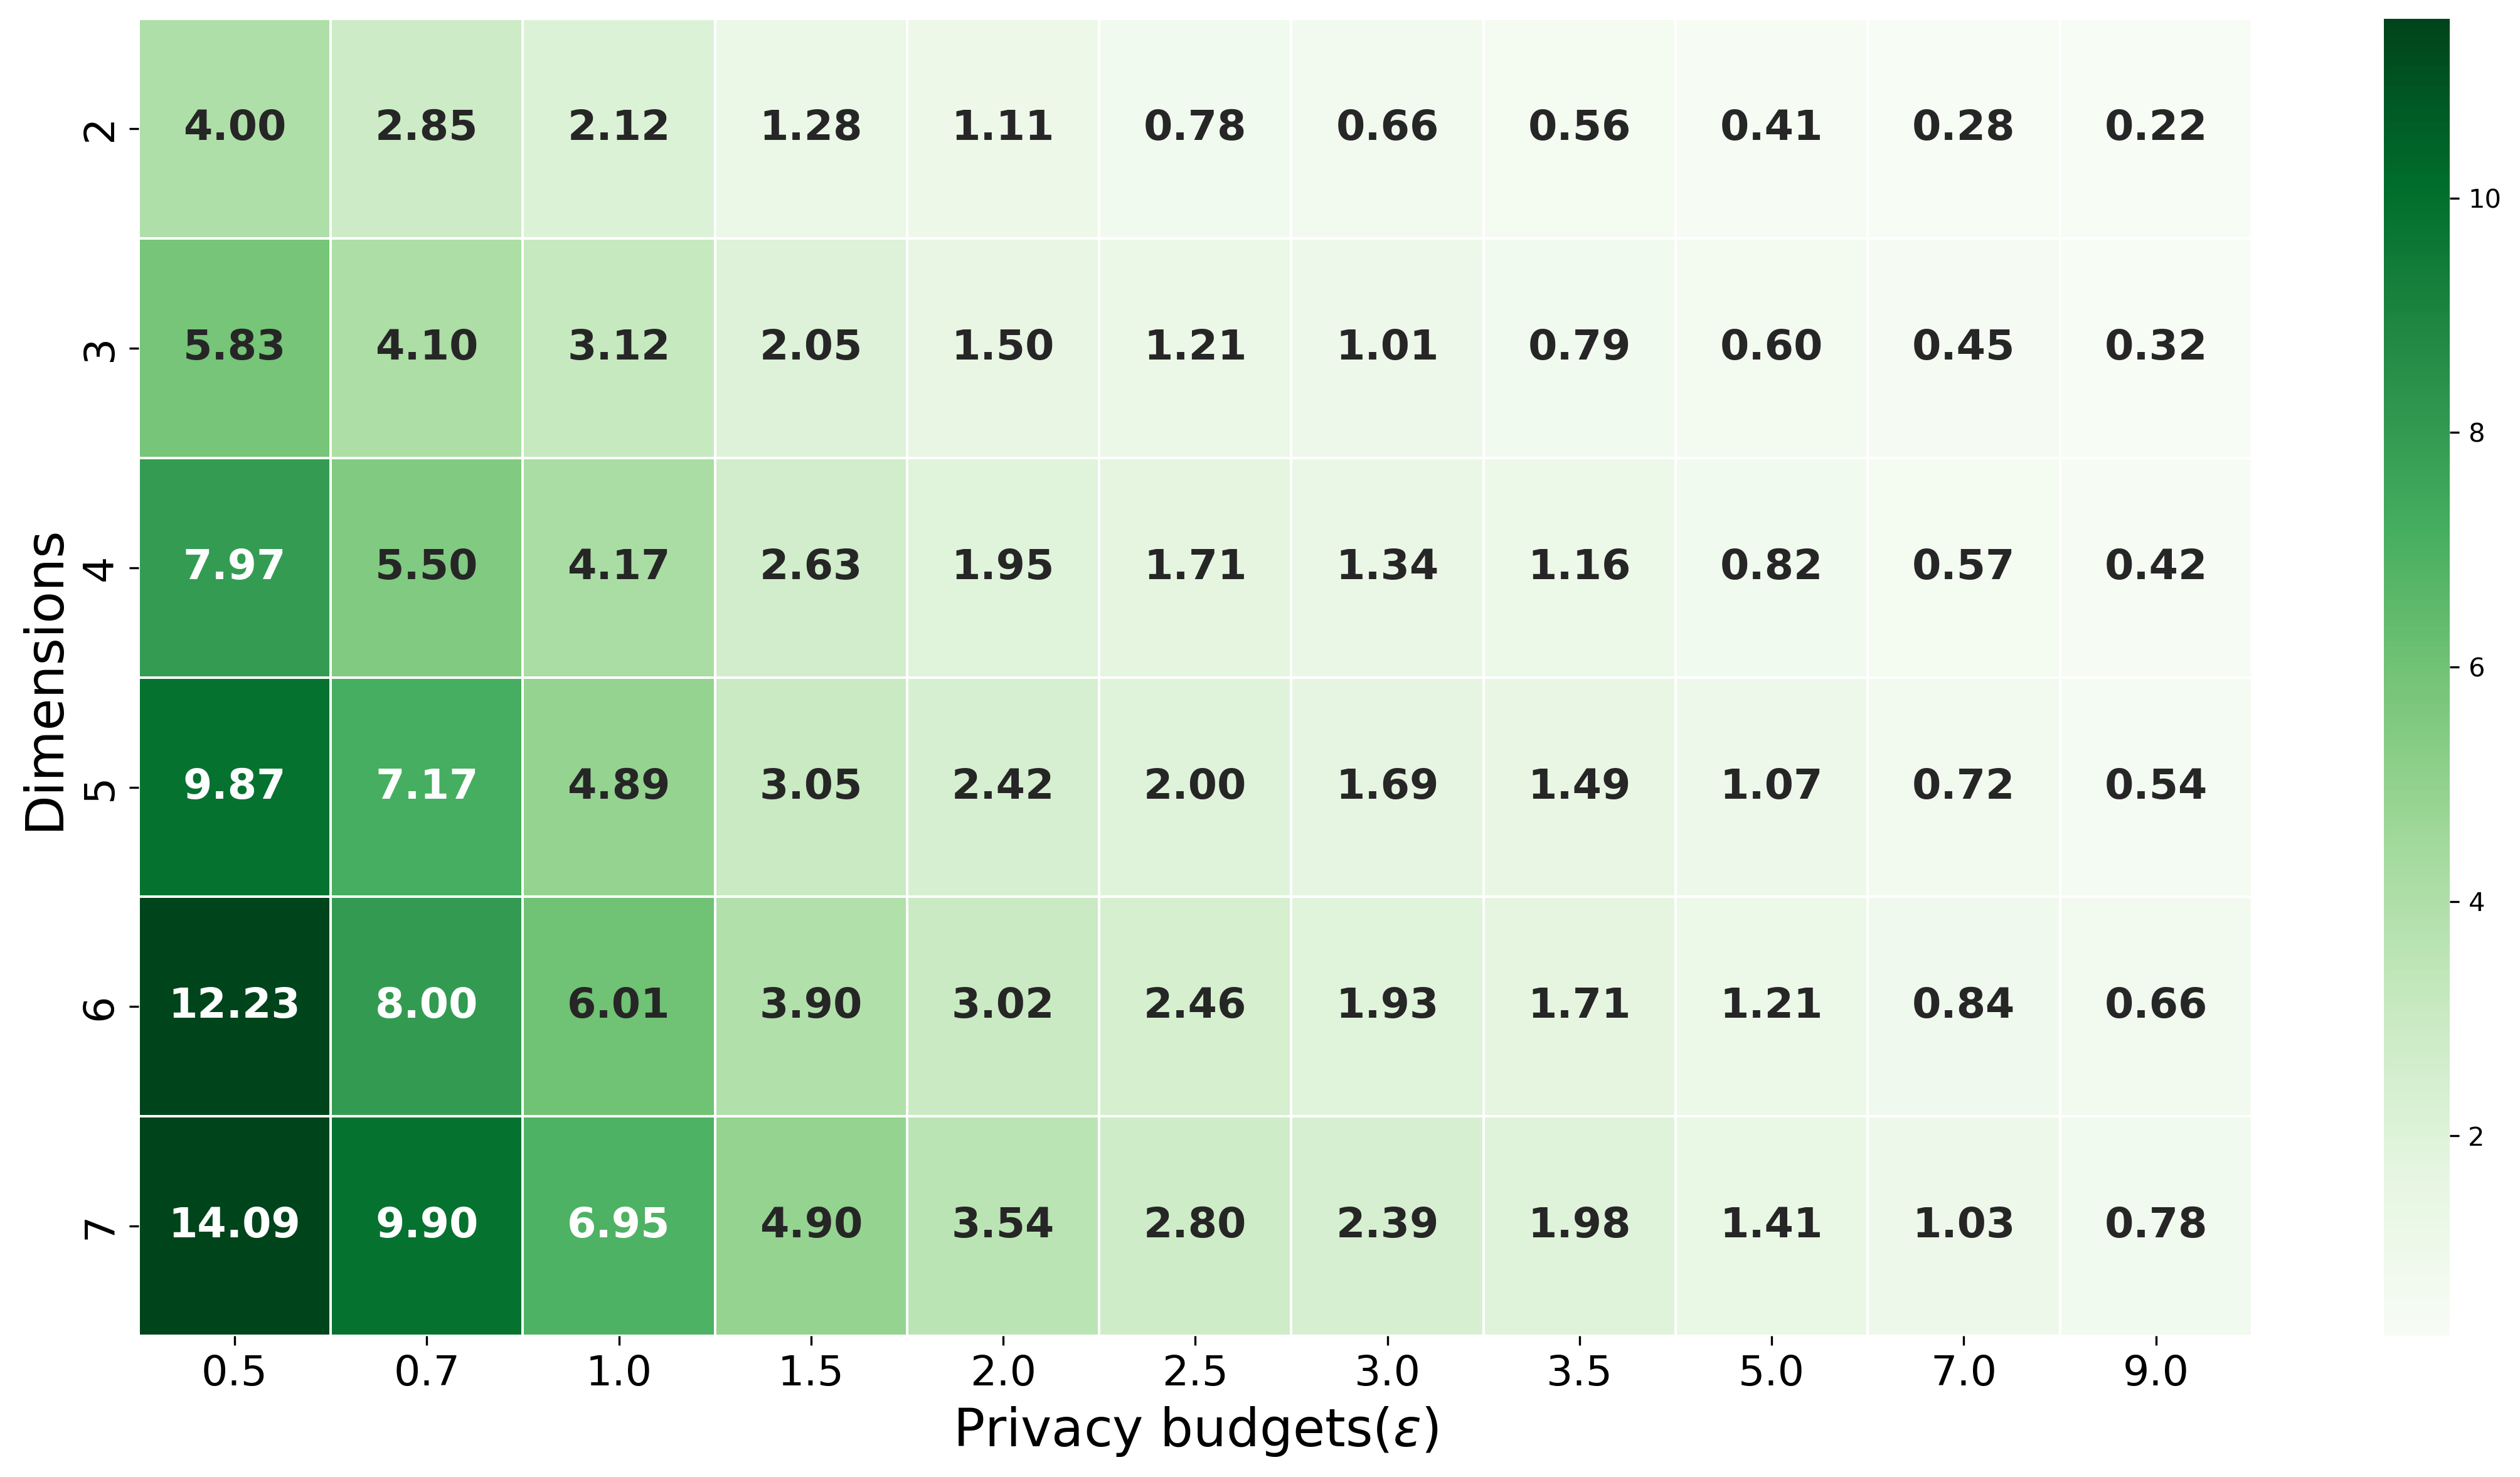
\includegraphics[width=1\textwidth]{Results/kd-laplace/kd-Laplace/seeds-dataset/distance.png}
            \label{fig:privacy_dist_seeds-dataset_adversial_advantage_kd-laplace}
        \end{subfigure}
        \vfill % vertical space

        \begin{subfigure}[c]{1\textwidth}
            \caption{\textbf{Heatmap showing disclosure risk for the Piecewise mechanism, per privacy budget \& dimension for seeds-dataset.}}
            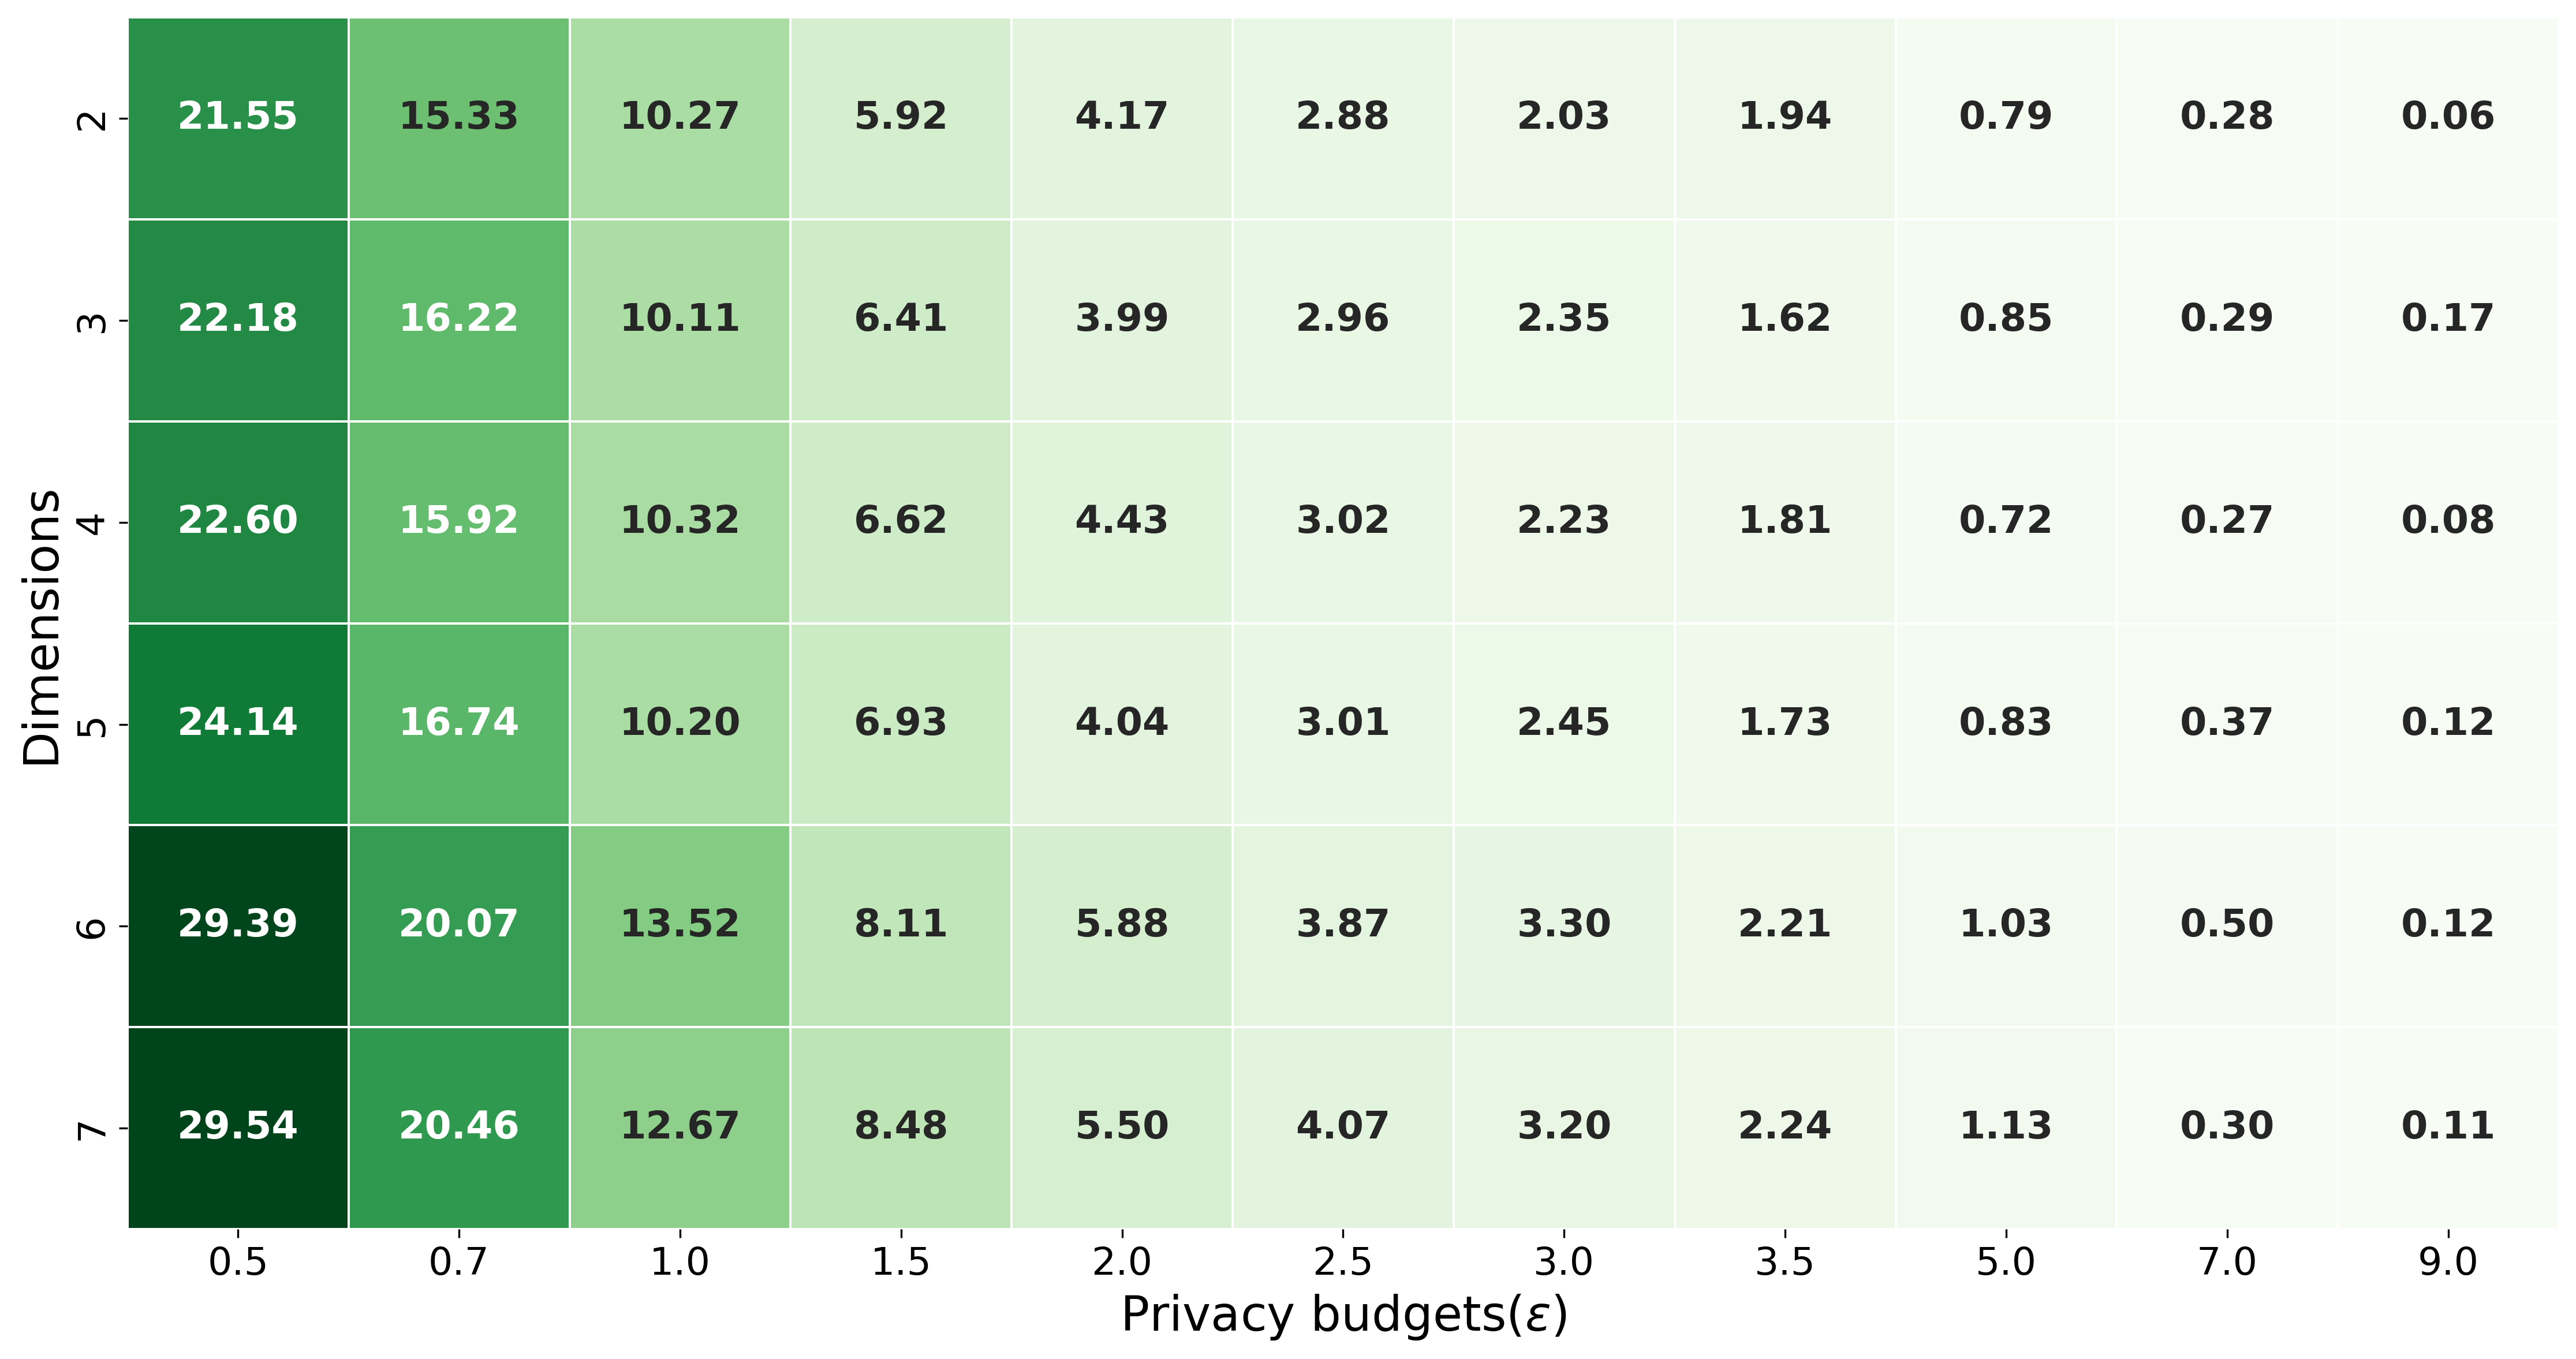
\includegraphics[width=1\textwidth]{Results/kd-laplace/piecewise/seeds-dataset/distance.png}
            \label{fig:privacy_dist_seeds-dataset_adversial_advantage_piecewise}
        \end{subfigure}
    \end{subfigure}
\end{figure}
\newpage

\todo[inline]{Add comments}
\subsection{Heart dataset} \label{appendix:results-privacy-heart-dataset}
\begin{figure}[H]
    \centering
    \begin{subfigure}[b]{0.85\textwidth}
        \begin{subfigure}[c]{1\textwidth}
            \caption{\textbf{Heatmap showing disclosure risk for the kD-Laplace mechanism, per privacy budget \& dimension for heart-dataset.}}
            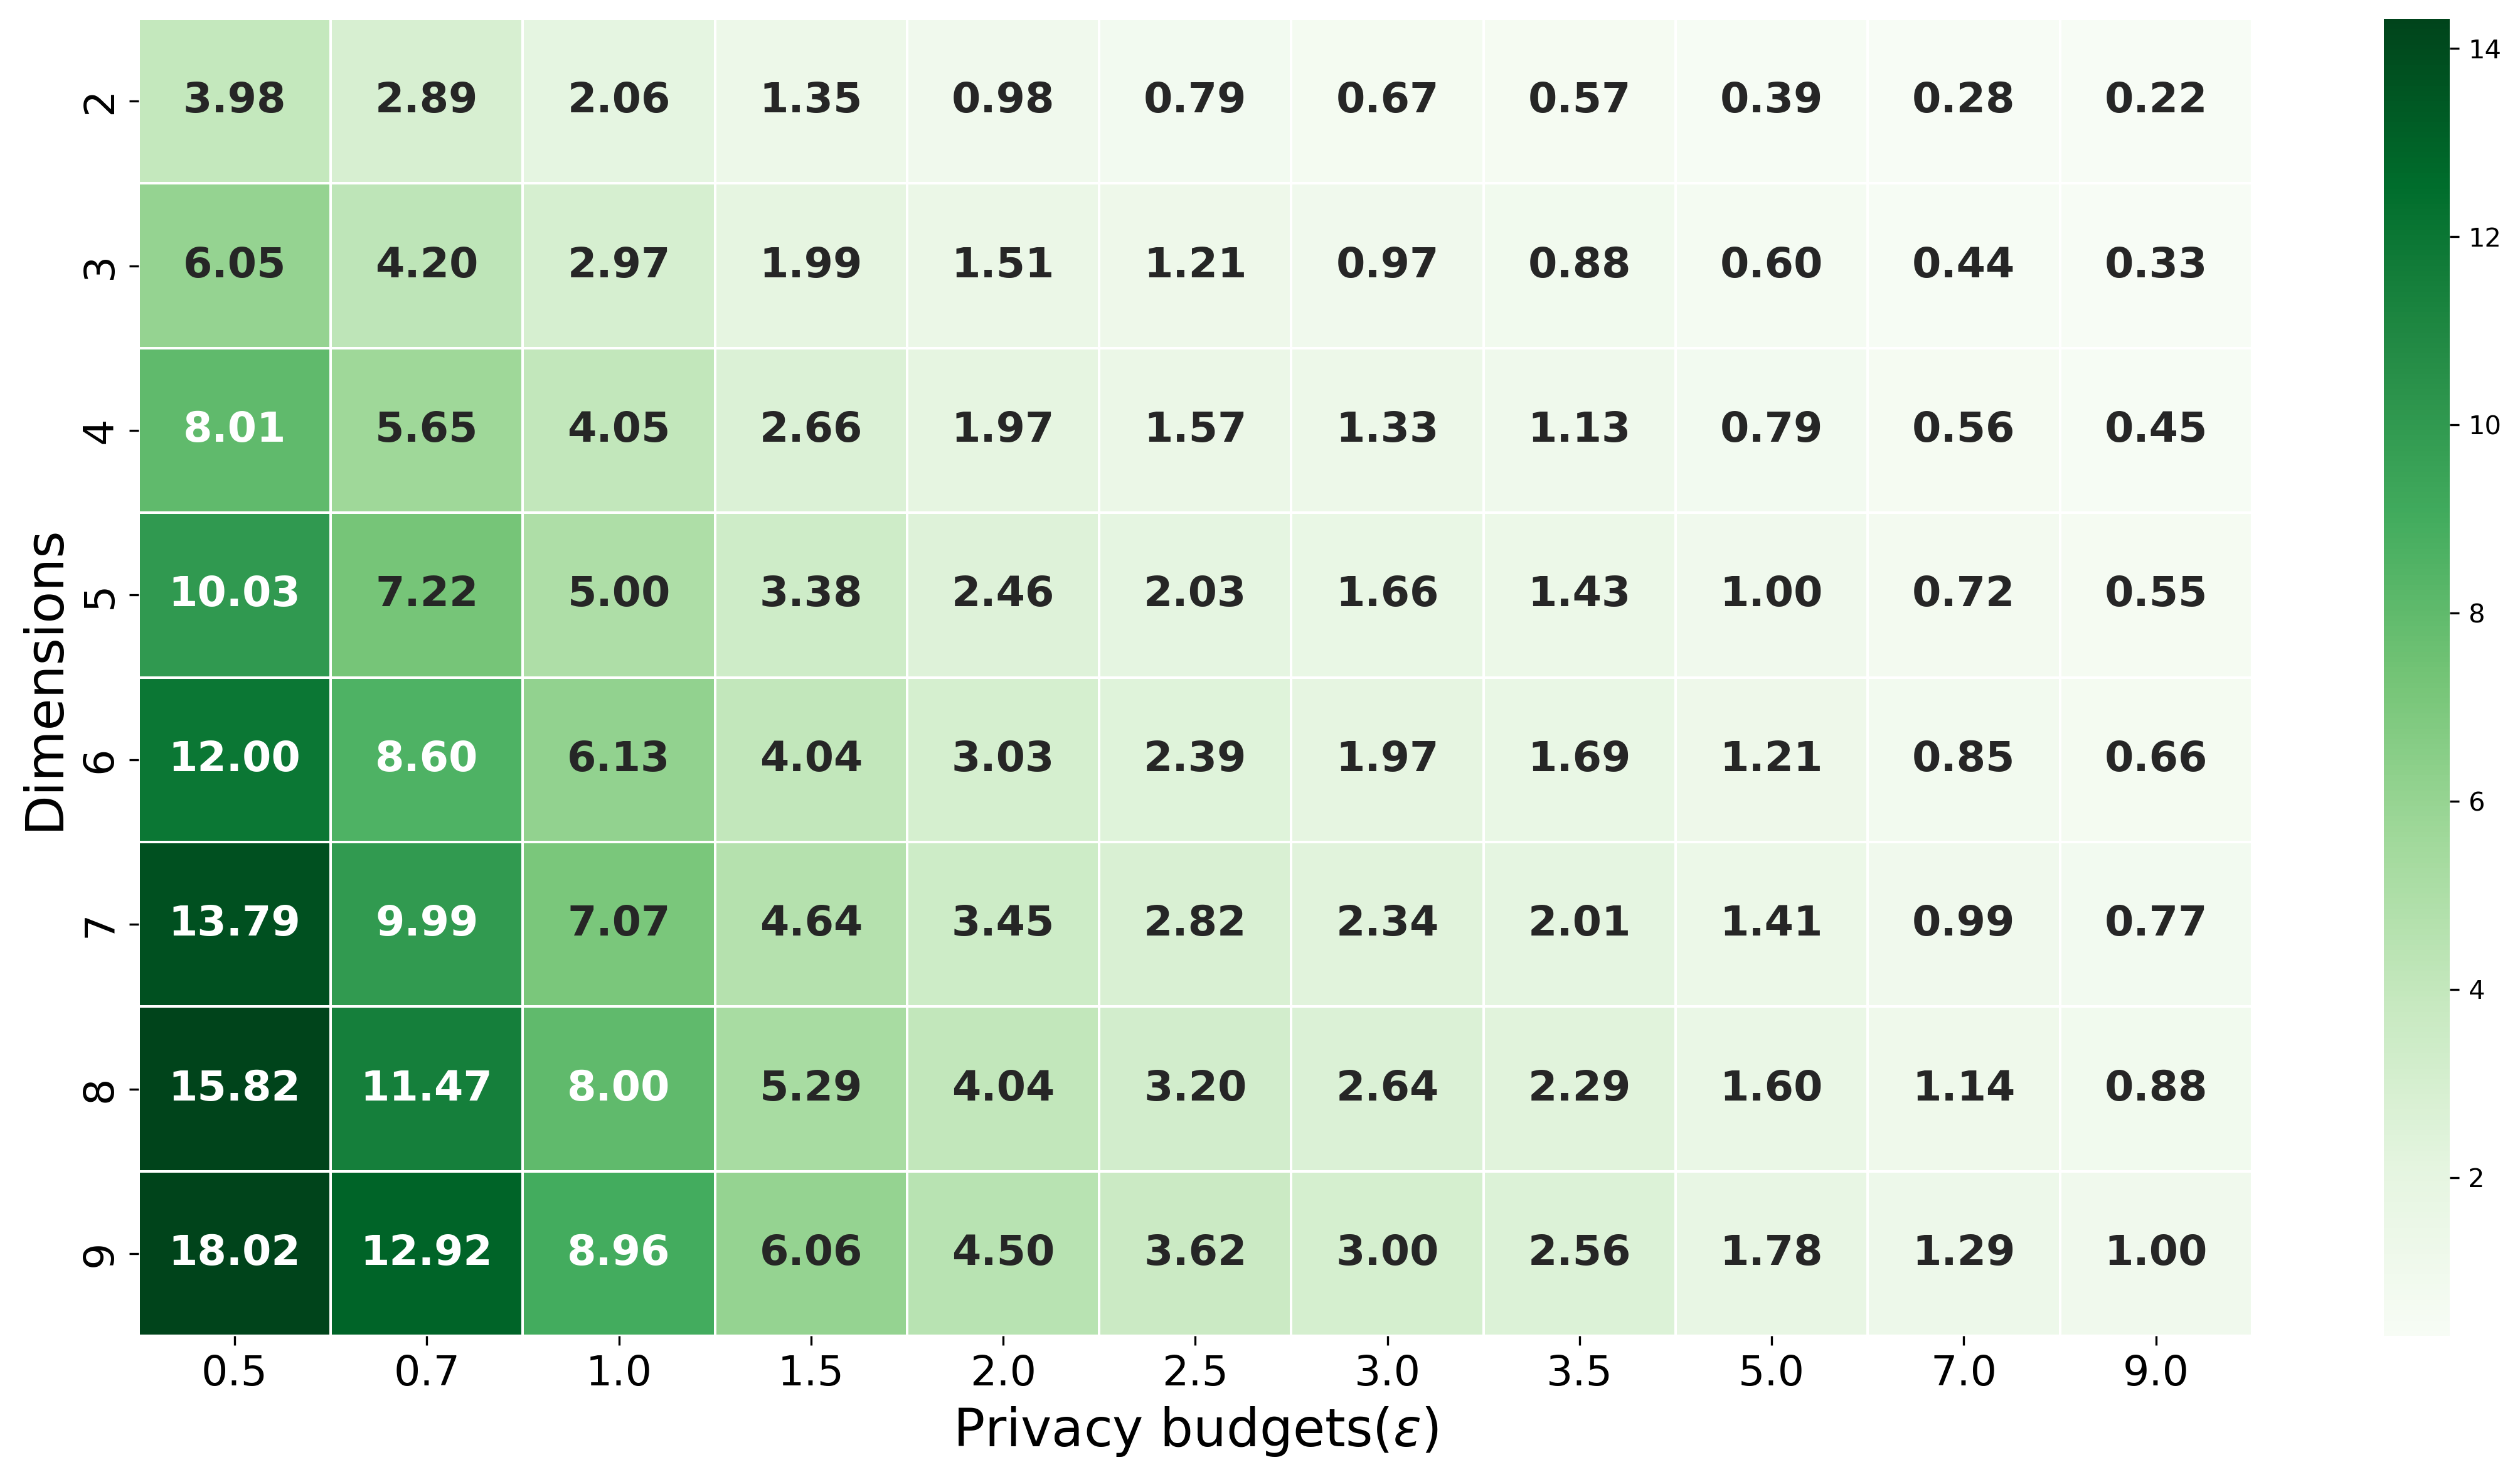
\includegraphics[width=1\textwidth]{Results/kd-laplace/kd-Laplace/heart-dataset/distance.png}
            \label{fig:privacy_risk_heart-dataset_adversial_advantage_kd-laplace}
        \end{subfigure}
        \vfill % vertical space

        \begin{subfigure}[c]{1\textwidth}
            \caption{\textbf{Heatmap showing disclosure risk for the Piecewise mechanism, per privacy budget \& dimension for heart-dataset.}}
            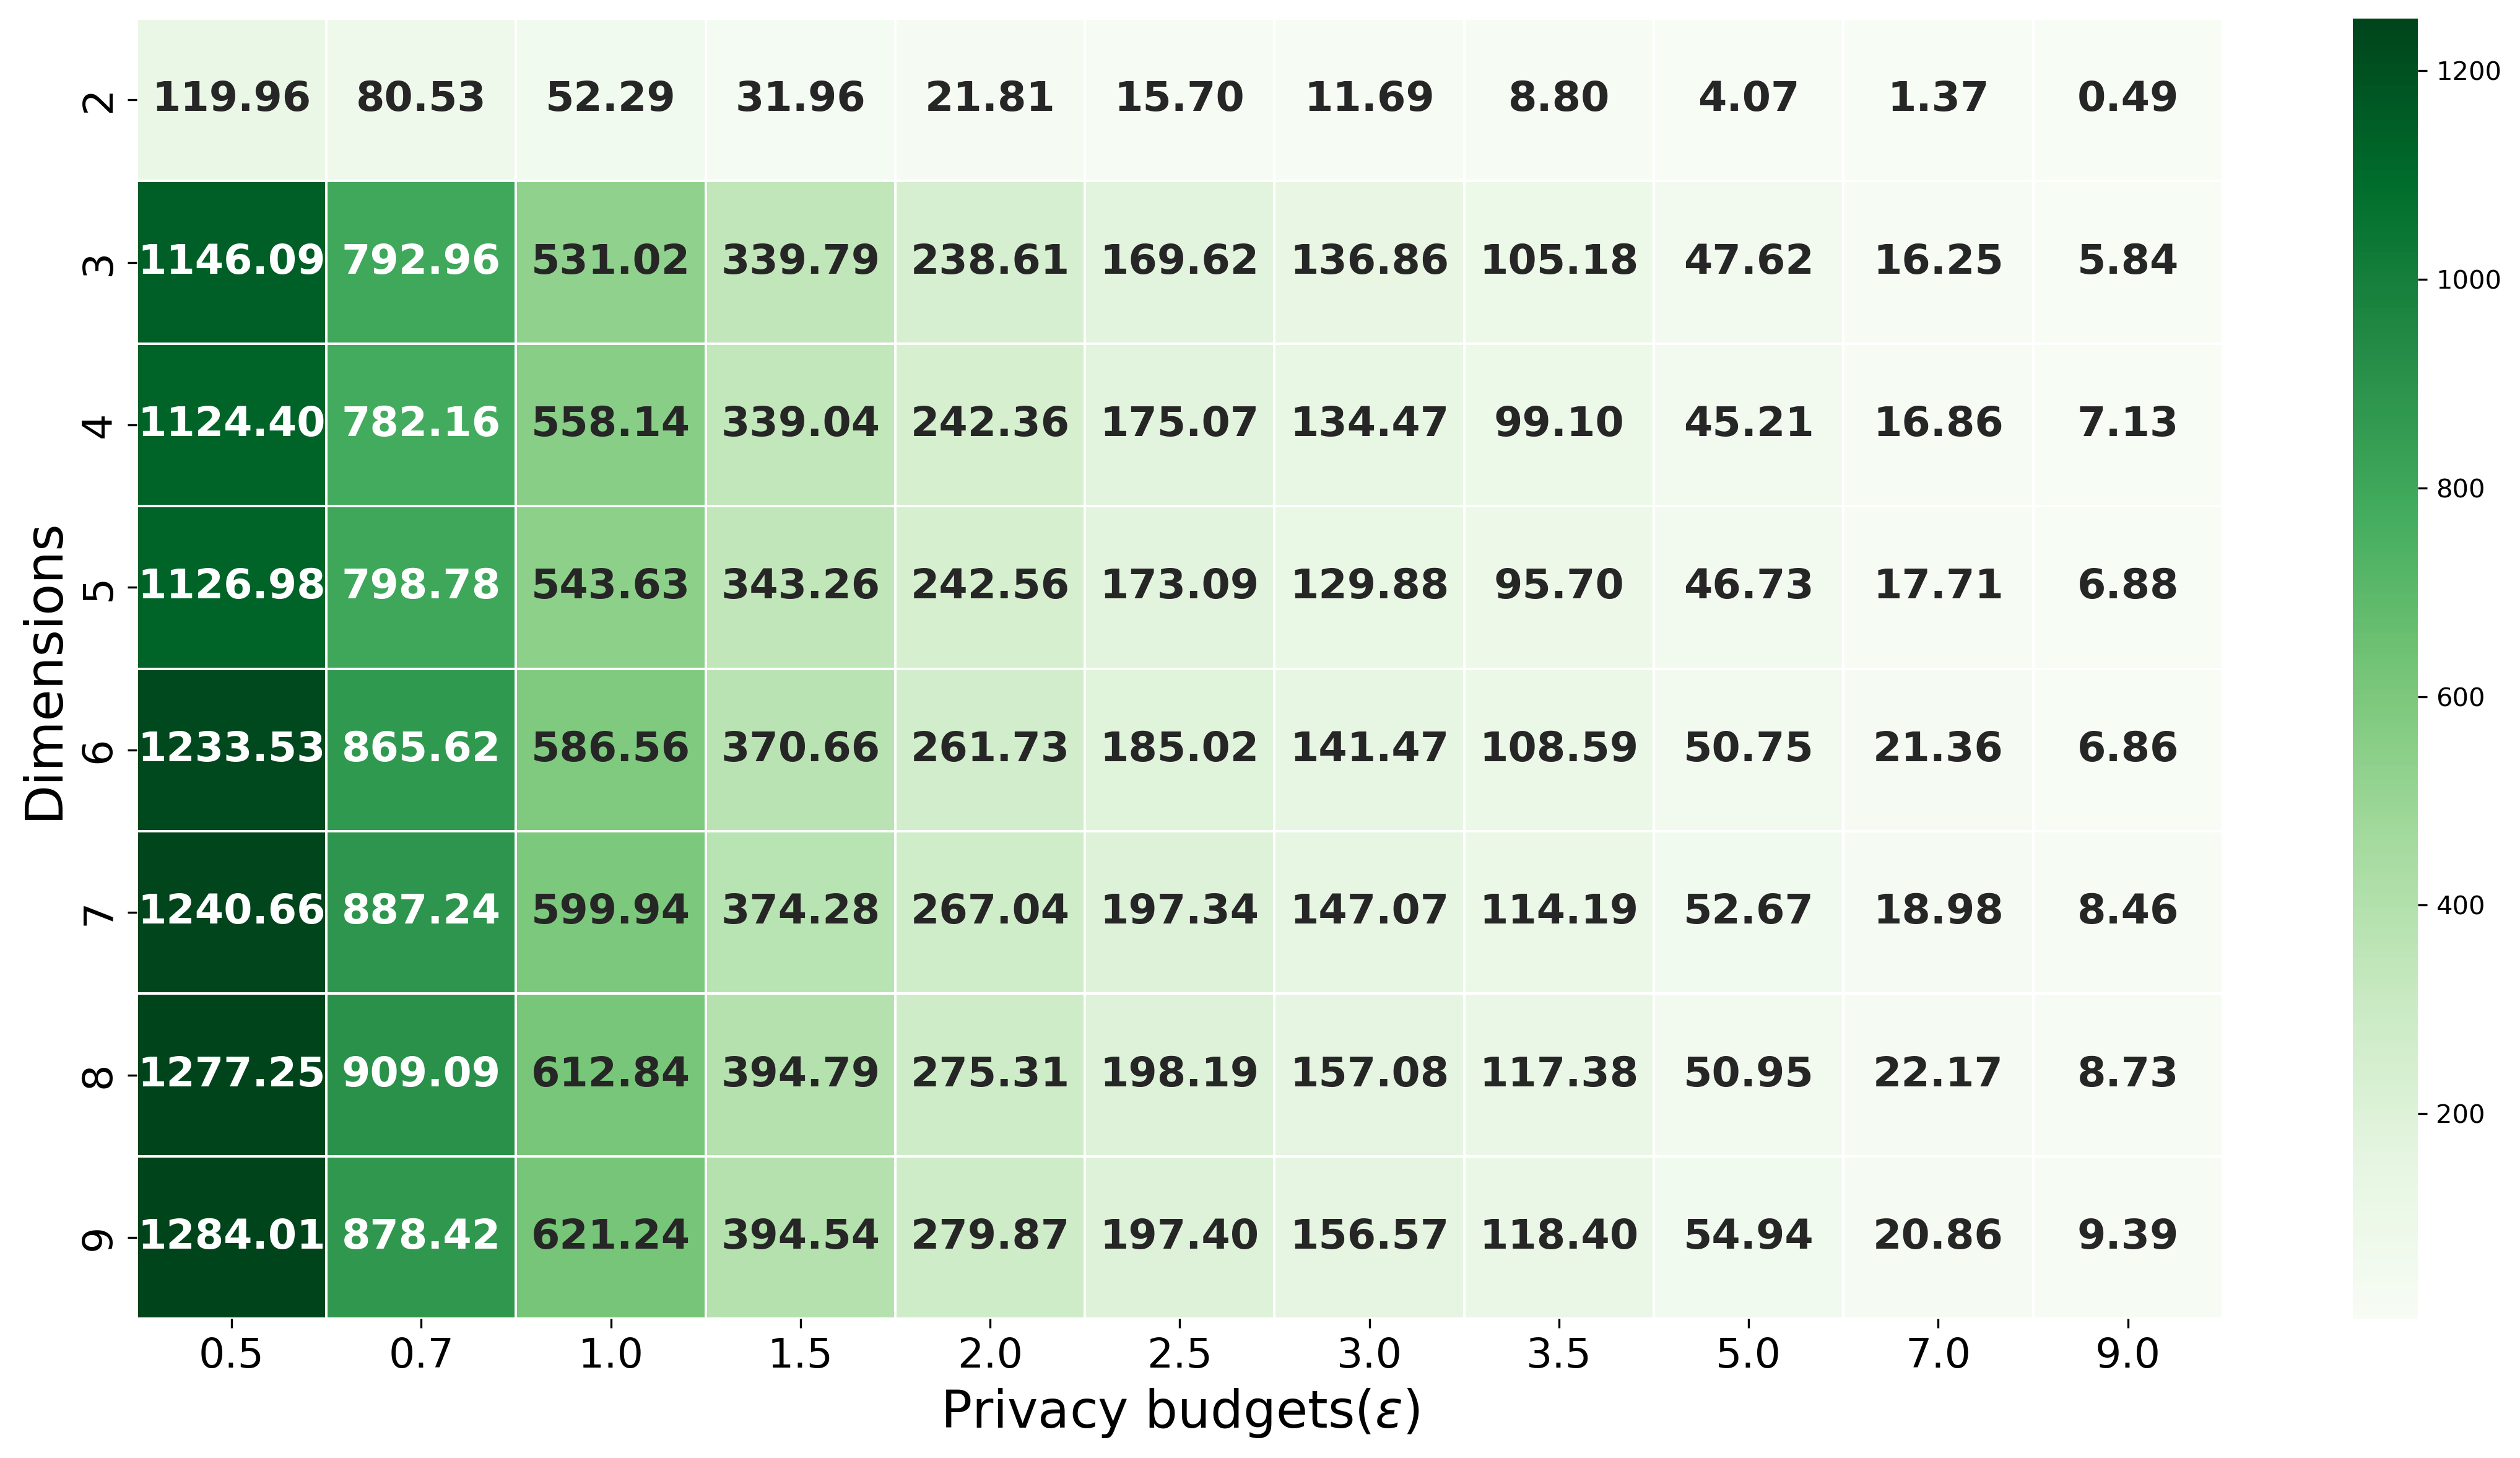
\includegraphics[width=1\textwidth]{Results/kd-laplace/piecewise/heart-dataset/distance.png}
            \label{fig:privacy_risk_heart-dataset_adversial_advantage_piecewise}
        \end{subfigure}
    \end{subfigure}
    \hfill % horizontal space
\end{figure}
\todo[inline]{Add comments}
\newpage

\todo[inline]{Add comments}
\newpage
\subsection{Circle dataset} \label{appendix:results-privacy-circle-dataset}
\begin{figure}
    \centering
    \begin{subfigure}[b]{0.85\textwidth}
        \begin{subfigure}[c]{1\textwidth}
            \caption{\textbf{Heatmap showing disclosure risk for the kD-Laplace mechanism, per privacy budget \& dimension for circle-dataset.}}
            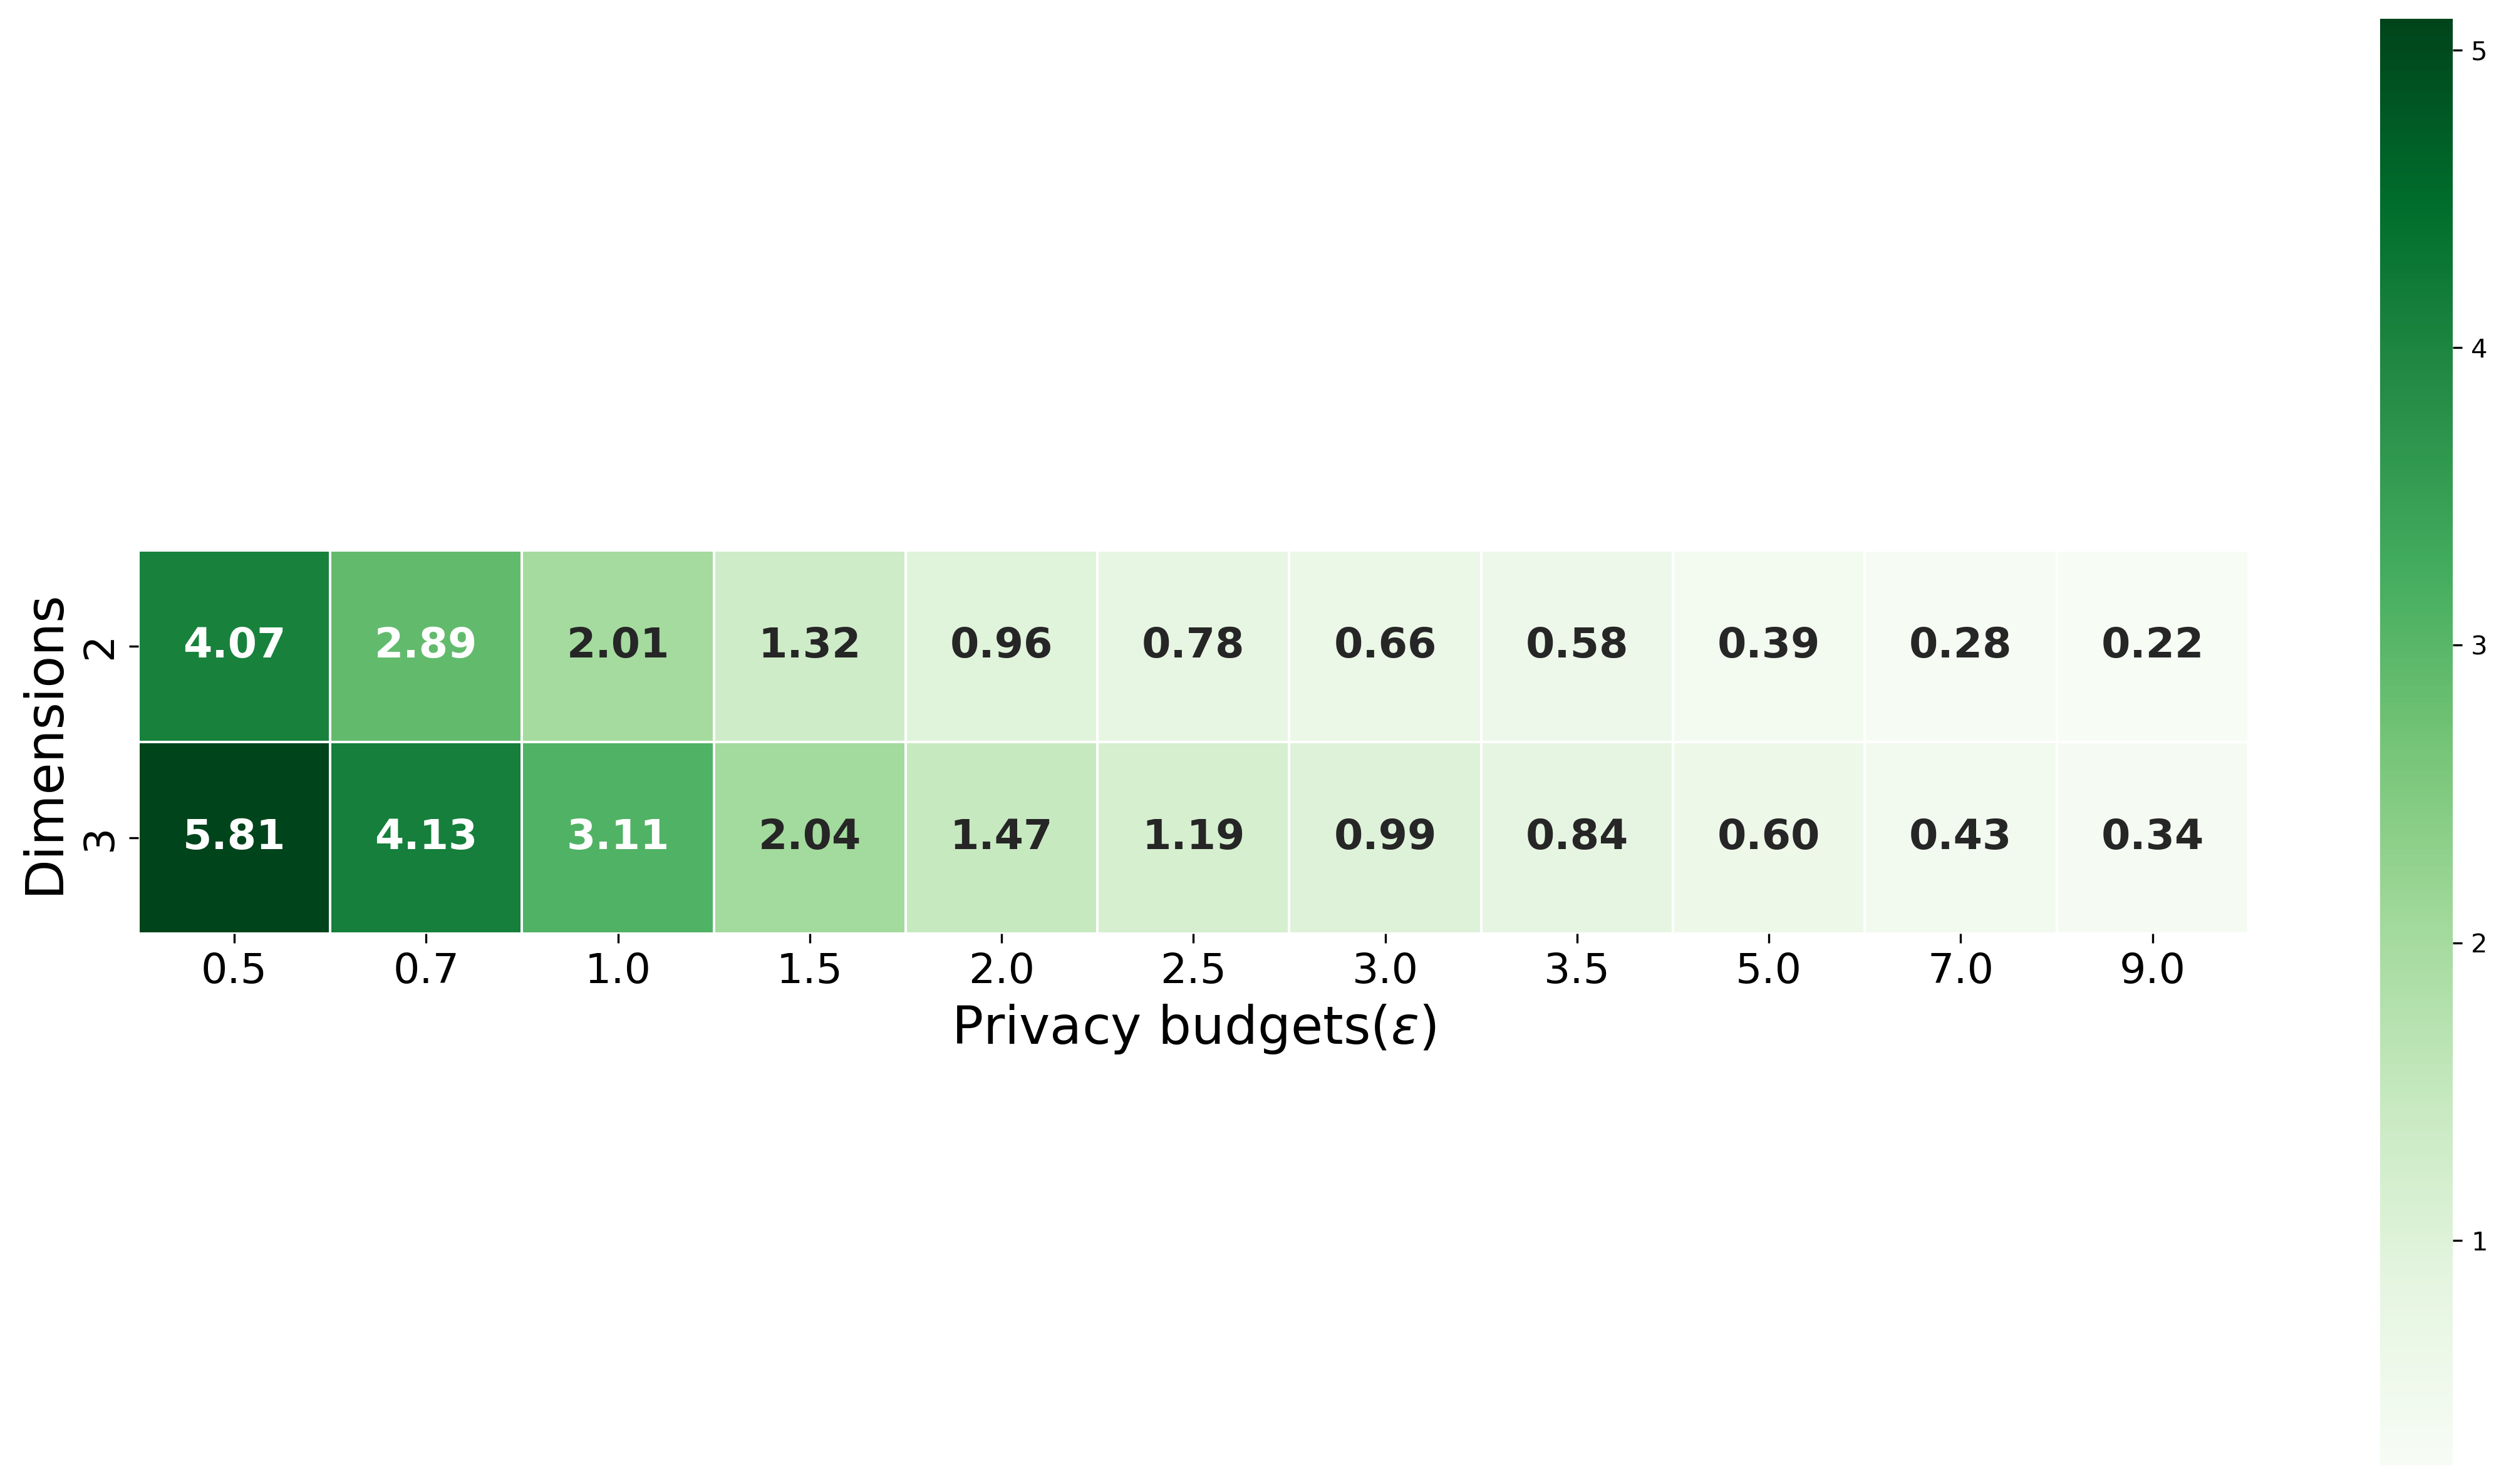
\includegraphics[width=1\textwidth]{Results/kd-laplace/kd-Laplace/circle-dataset/distance.png}
            \label{fig:privacy-risk_circle-dataset_adversial_advantage_kd-laplace}
        \end{subfigure}
        \vfill % vertical space

        \begin{subfigure}[c]{1\textwidth}
            \caption{\textbf{Heatmap showing disclosure risk for the Piecewise mechanism, per privacy budget \& dimension for circle-dataset.}}
            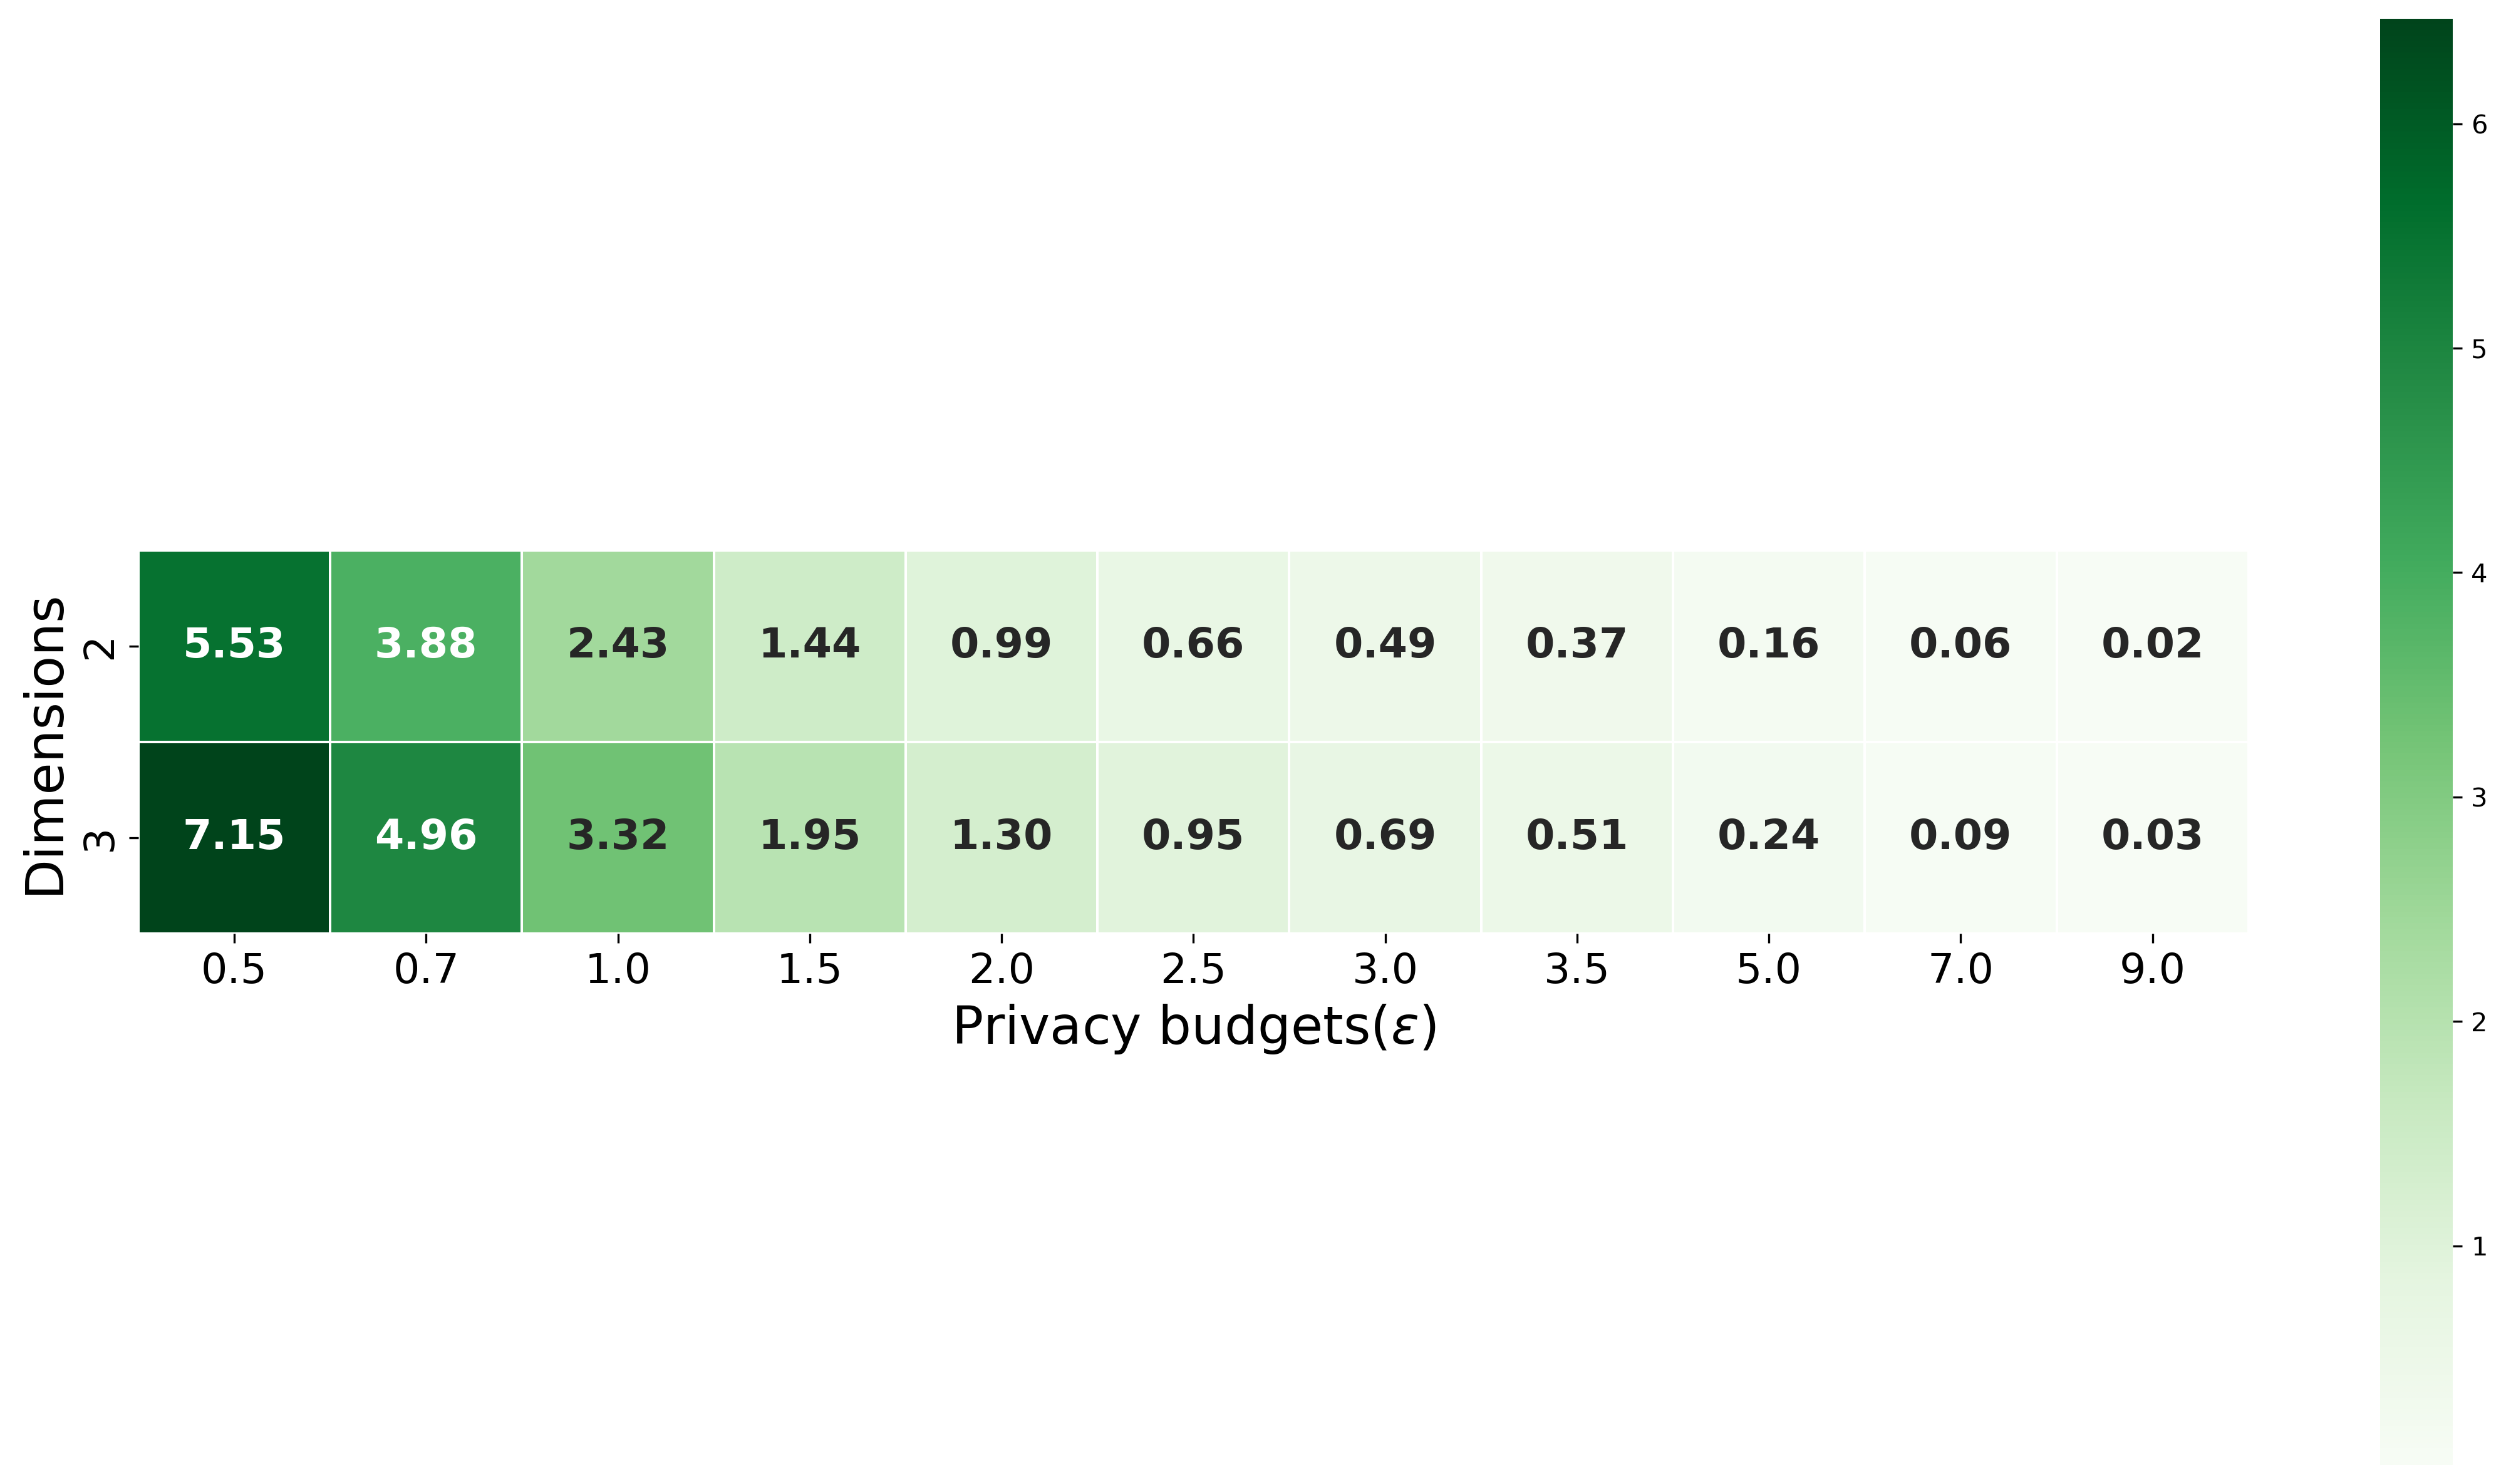
\includegraphics[width=1\textwidth]{Results/kd-laplace/piecewise/circle-dataset/distance.png}
            \label{fig:privacy-risk_circle-dataset_adversial_advantage_piecewise}
        \end{subfigure}
    \end{subfigure}
\end{figure}
\todo[inline]{Add comments}
\newpage
\subsection{Line dataset} \label{appendix:results-privacy-line-dataset}
\begin{figure}
    \centering
    \begin{subfigure}[b]{0.85\textwidth}
        \begin{subfigure}[c]{1\textwidth}
            \caption{\textbf{Heatmap showing disclosure risk for the kD-Laplace mechanism, per privacy budget \& dimension for line-dataset.}}
            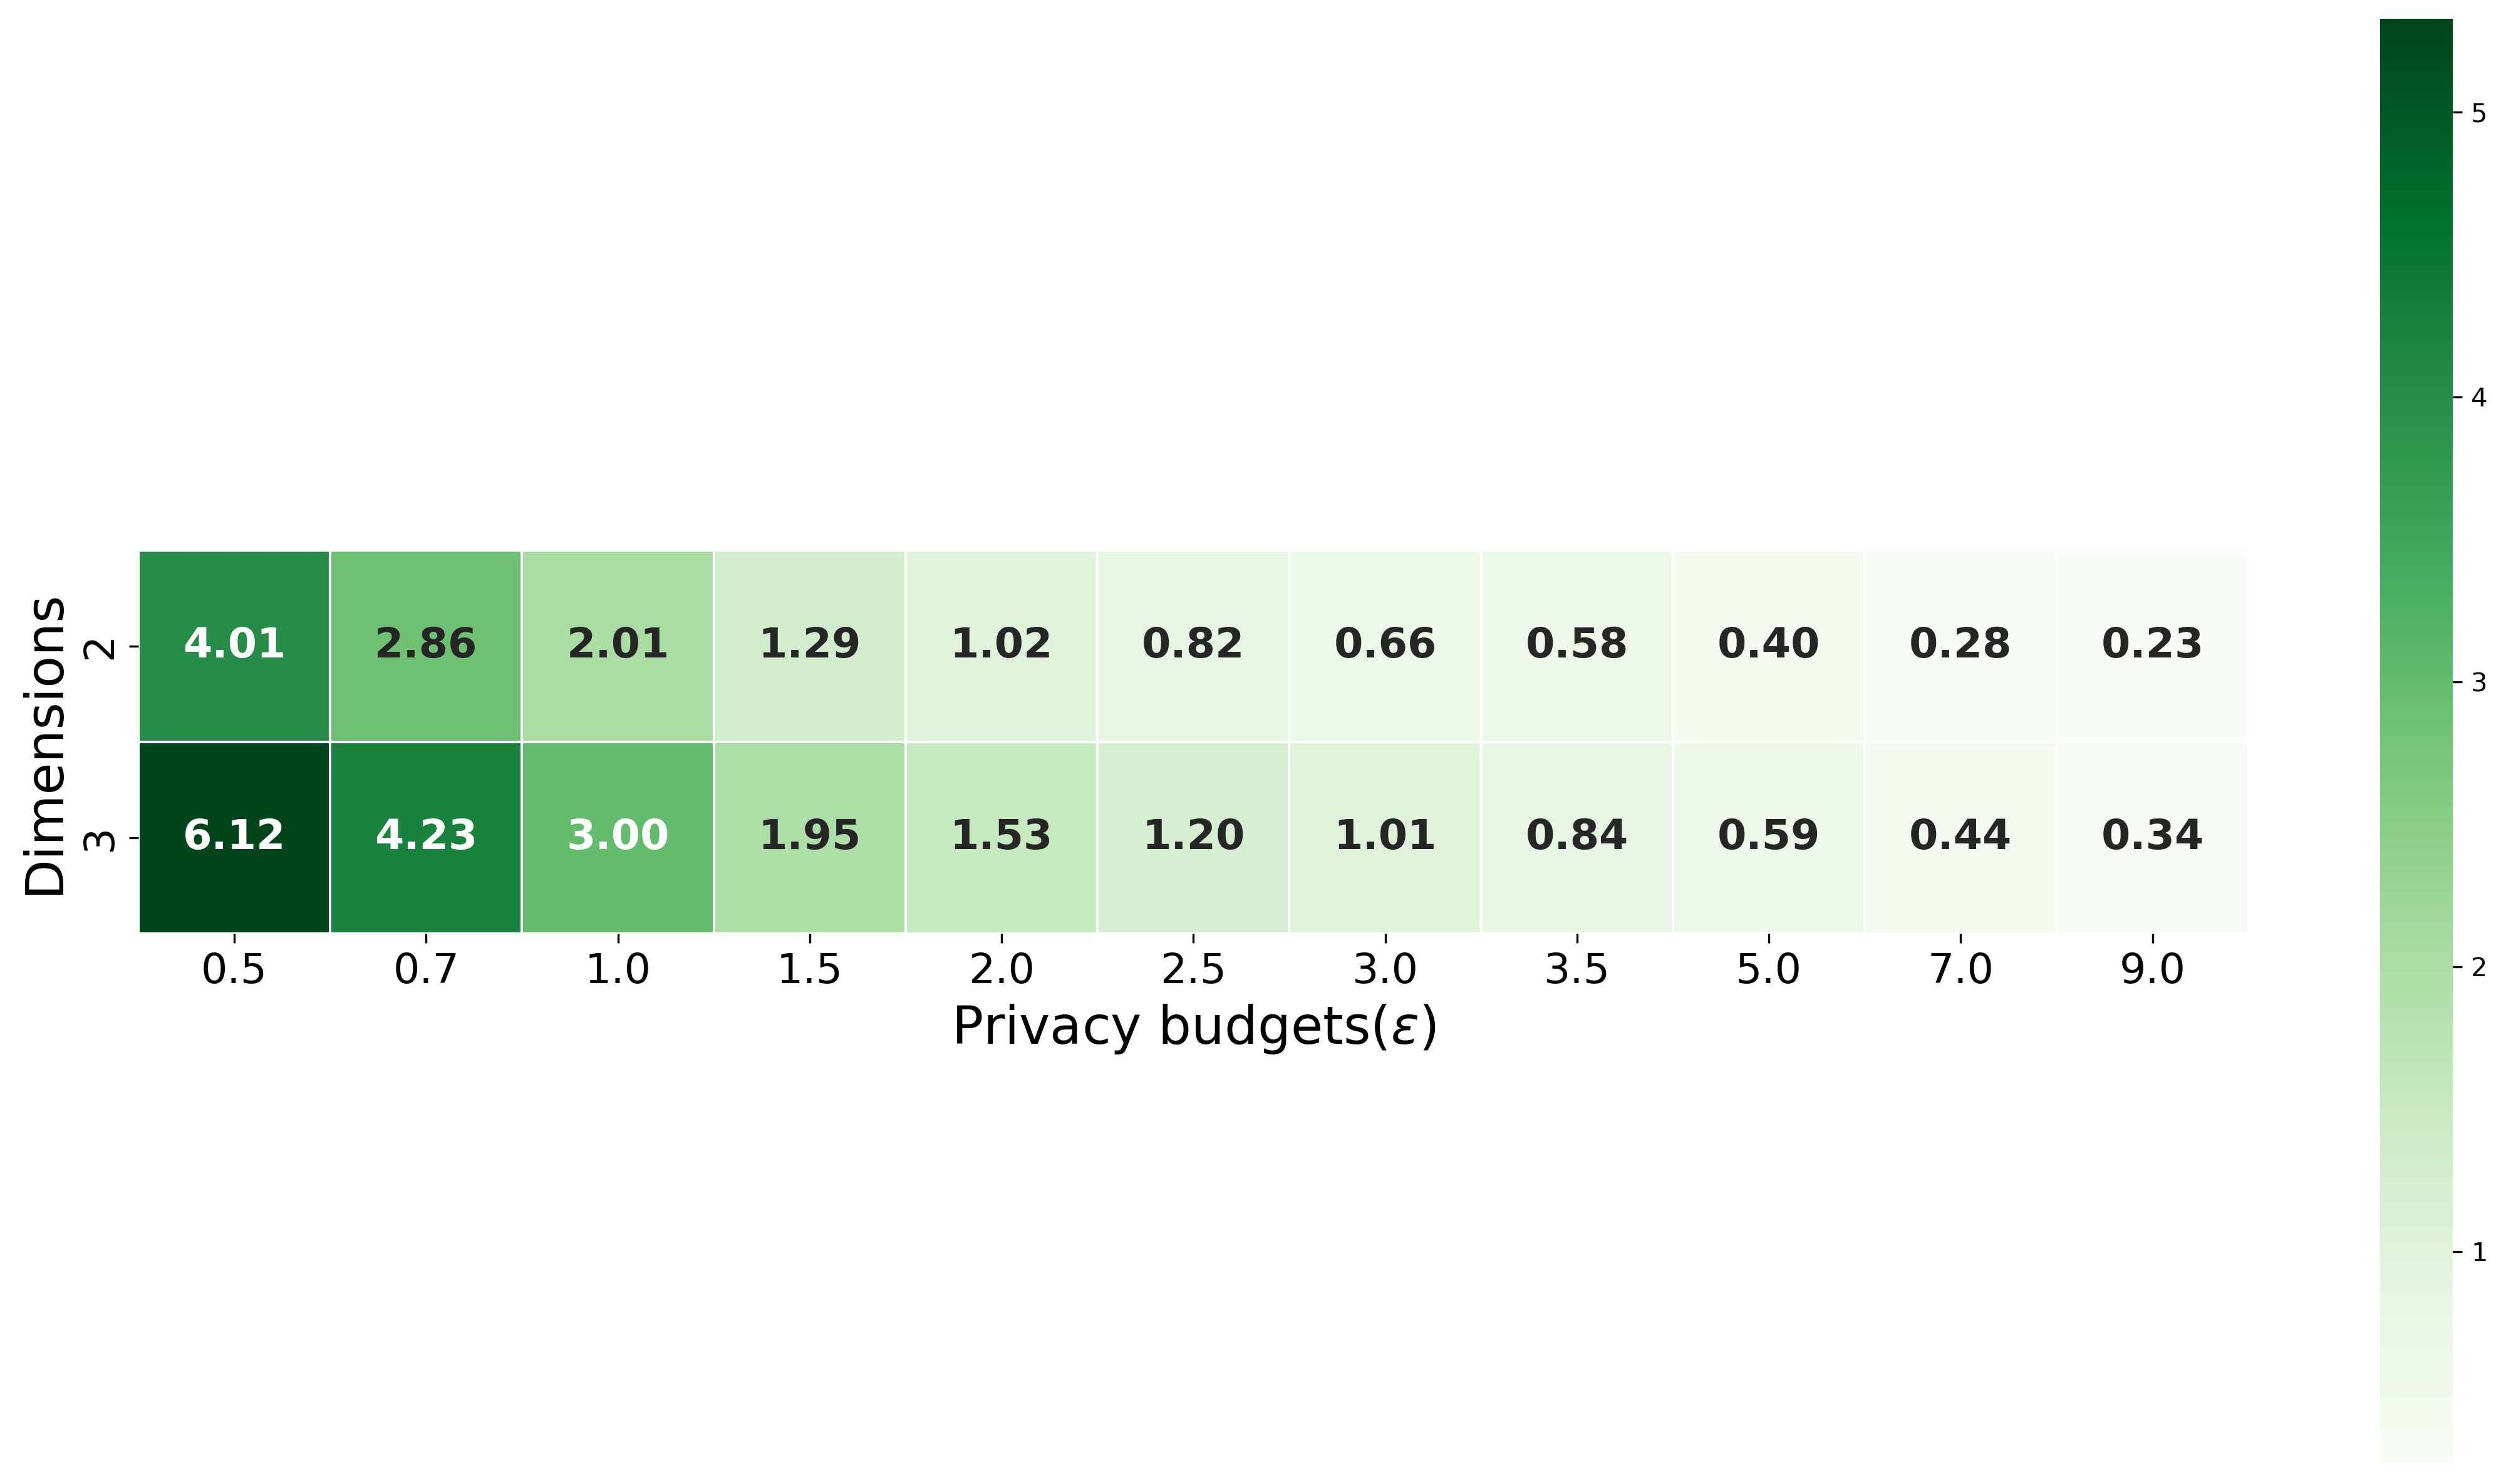
\includegraphics[width=1\textwidth]{Results/kd-laplace/kd-Laplace/line-dataset/distance.png}
            \label{fig:privacy-risk_line-dataset_adversial_advantage_kd-laplace}
        \end{subfigure}
        \vfill % vertical space

        \begin{subfigure}[c]{1\textwidth}
            \caption{\textbf{Heatmap showing disclosure risk for the Piecewise mechanism, per privacy budget \& dimension for line-dataset.}}
            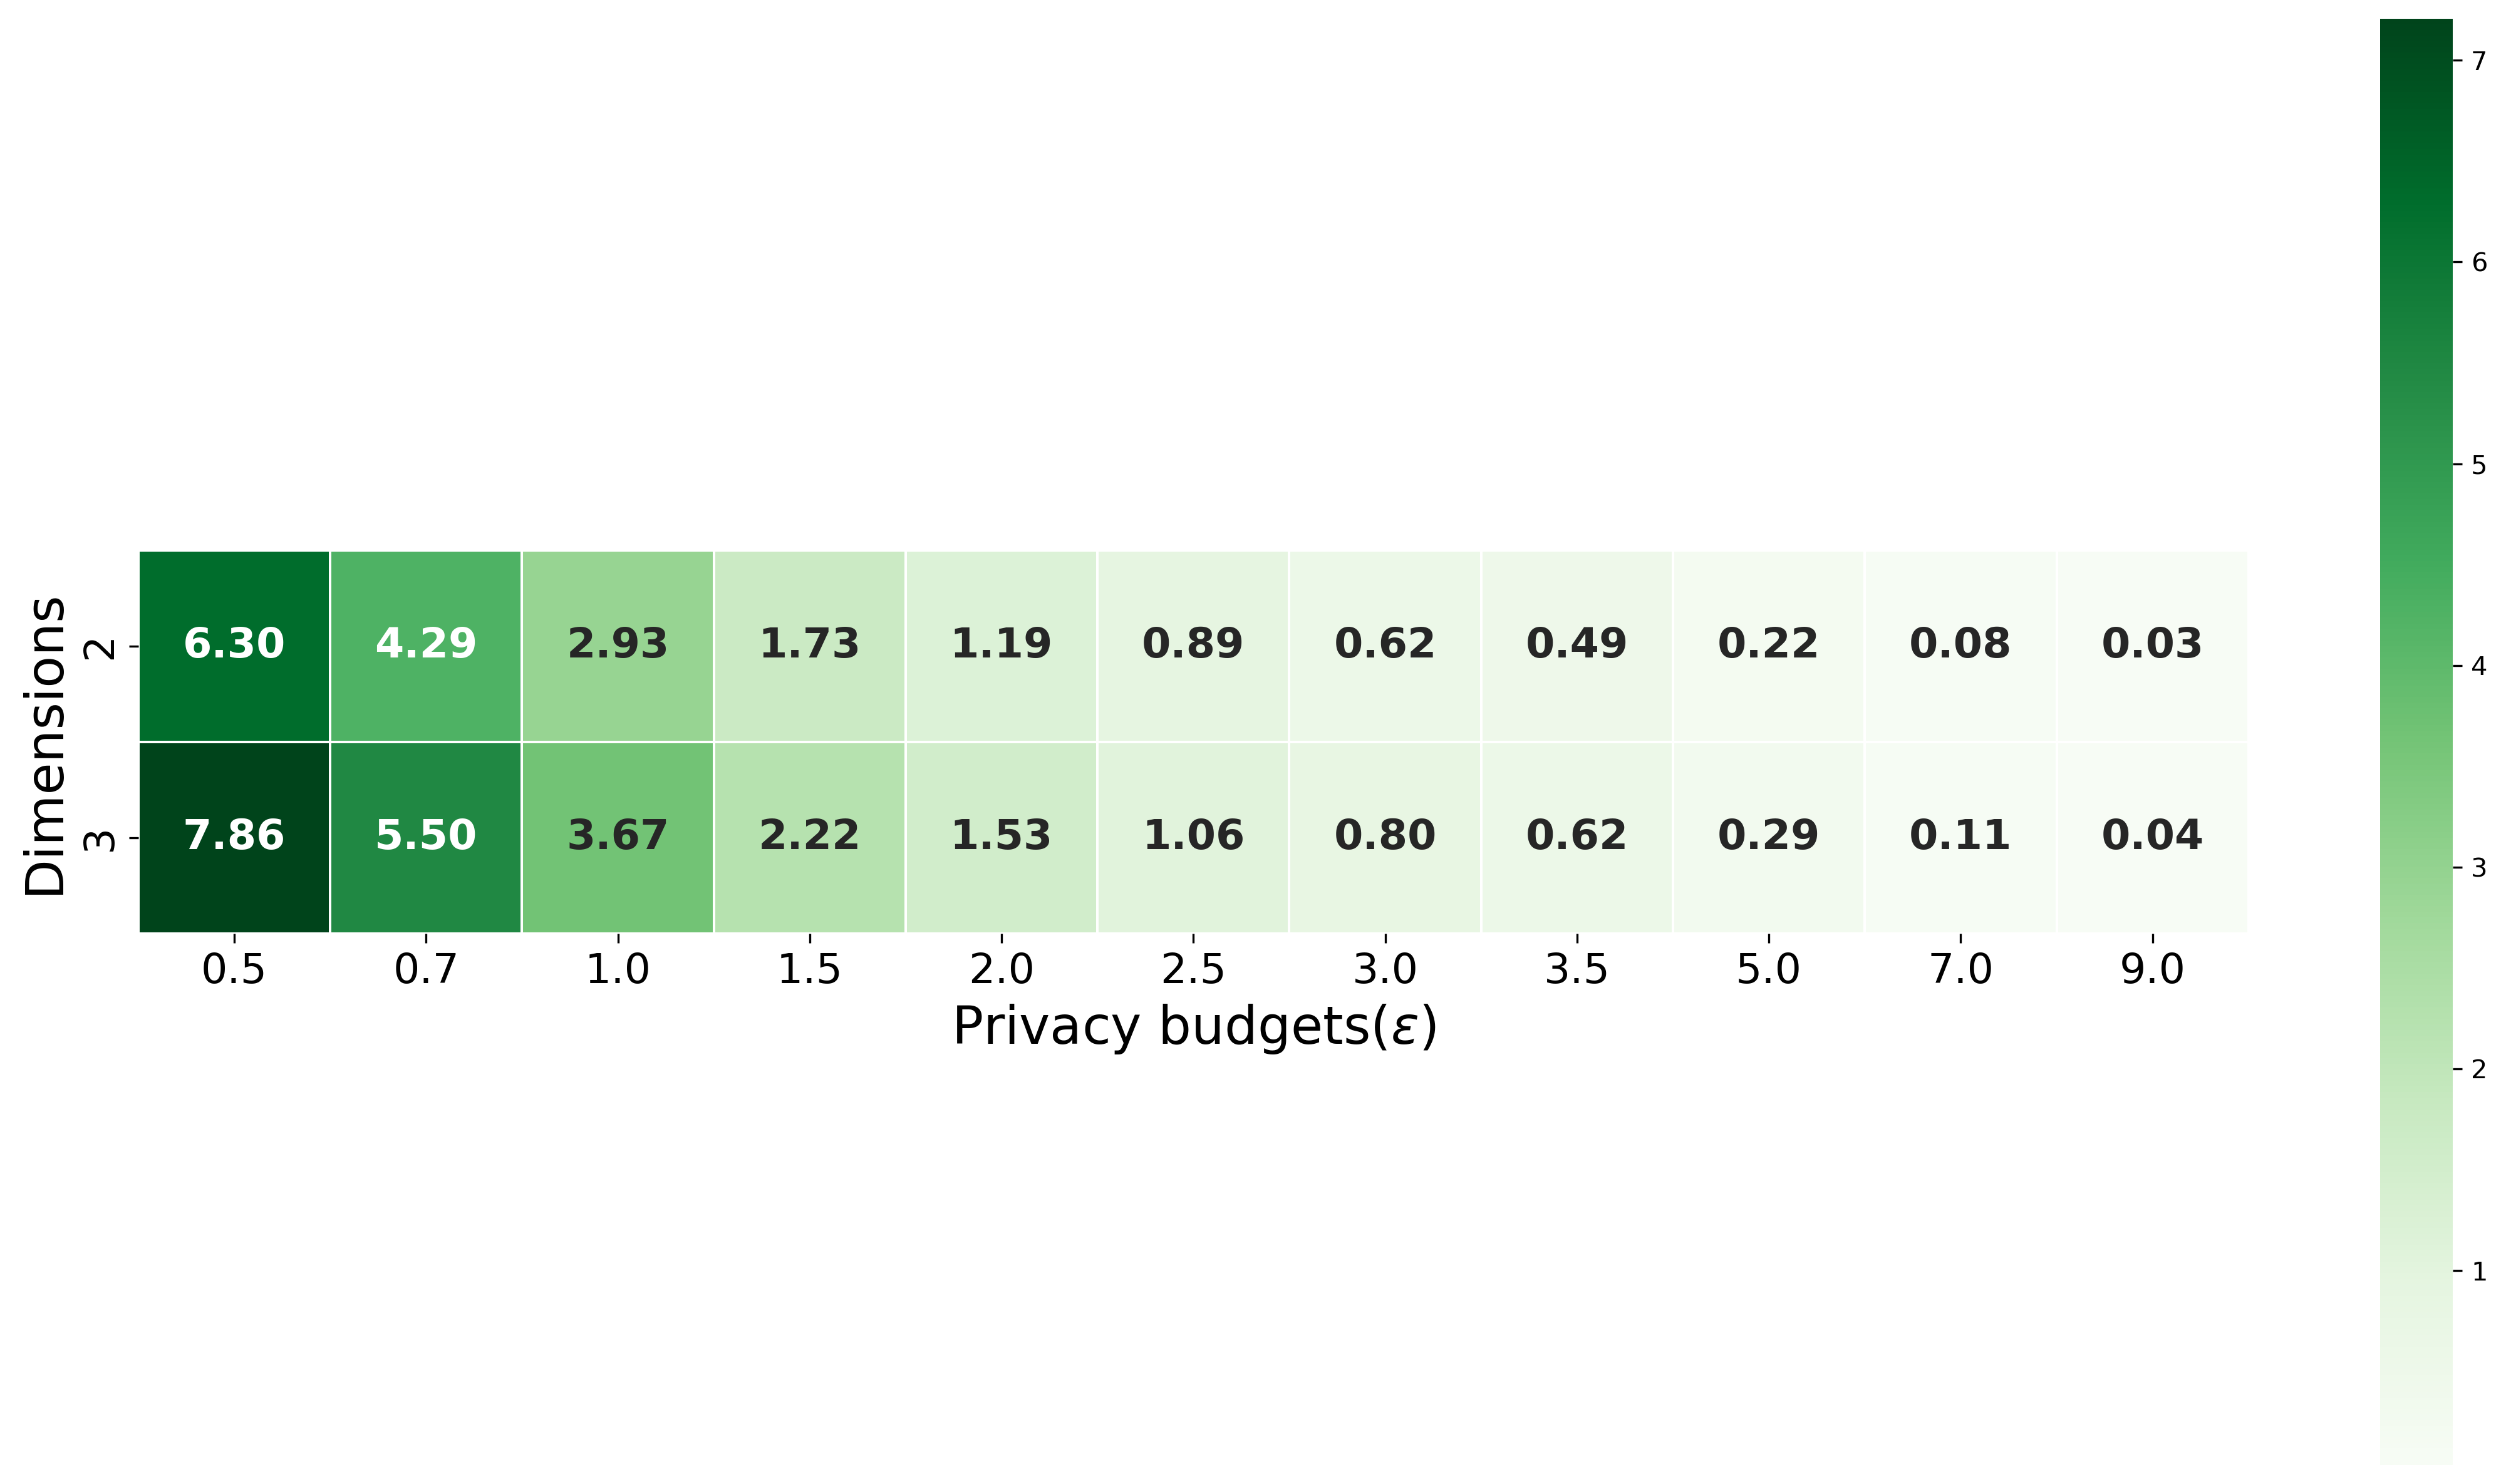
\includegraphics[width=1\textwidth]{Results/kd-laplace/piecewise/line-dataset/distance.png}
            \label{fig:privacy-risk_line-dataset_adversial_advantage_piecewise}
        \end{subfigure}
    \end{subfigure}
\end{figure}
\todo[inline]{Add comments}
\newpage
\subsection{Skewed dataset} \label{appendix:results-privacy-skewed-dataset}
\begin{figure}
    \centering
    \begin{subfigure}[b]{0.85\textwidth}
        \begin{subfigure}[c]{1\textwidth}
            \caption{\textbf{Heatmap showing disclosure risk for the kD-Laplace mechanism, per privacy budget \& dimension for skewed-dataset.}}
            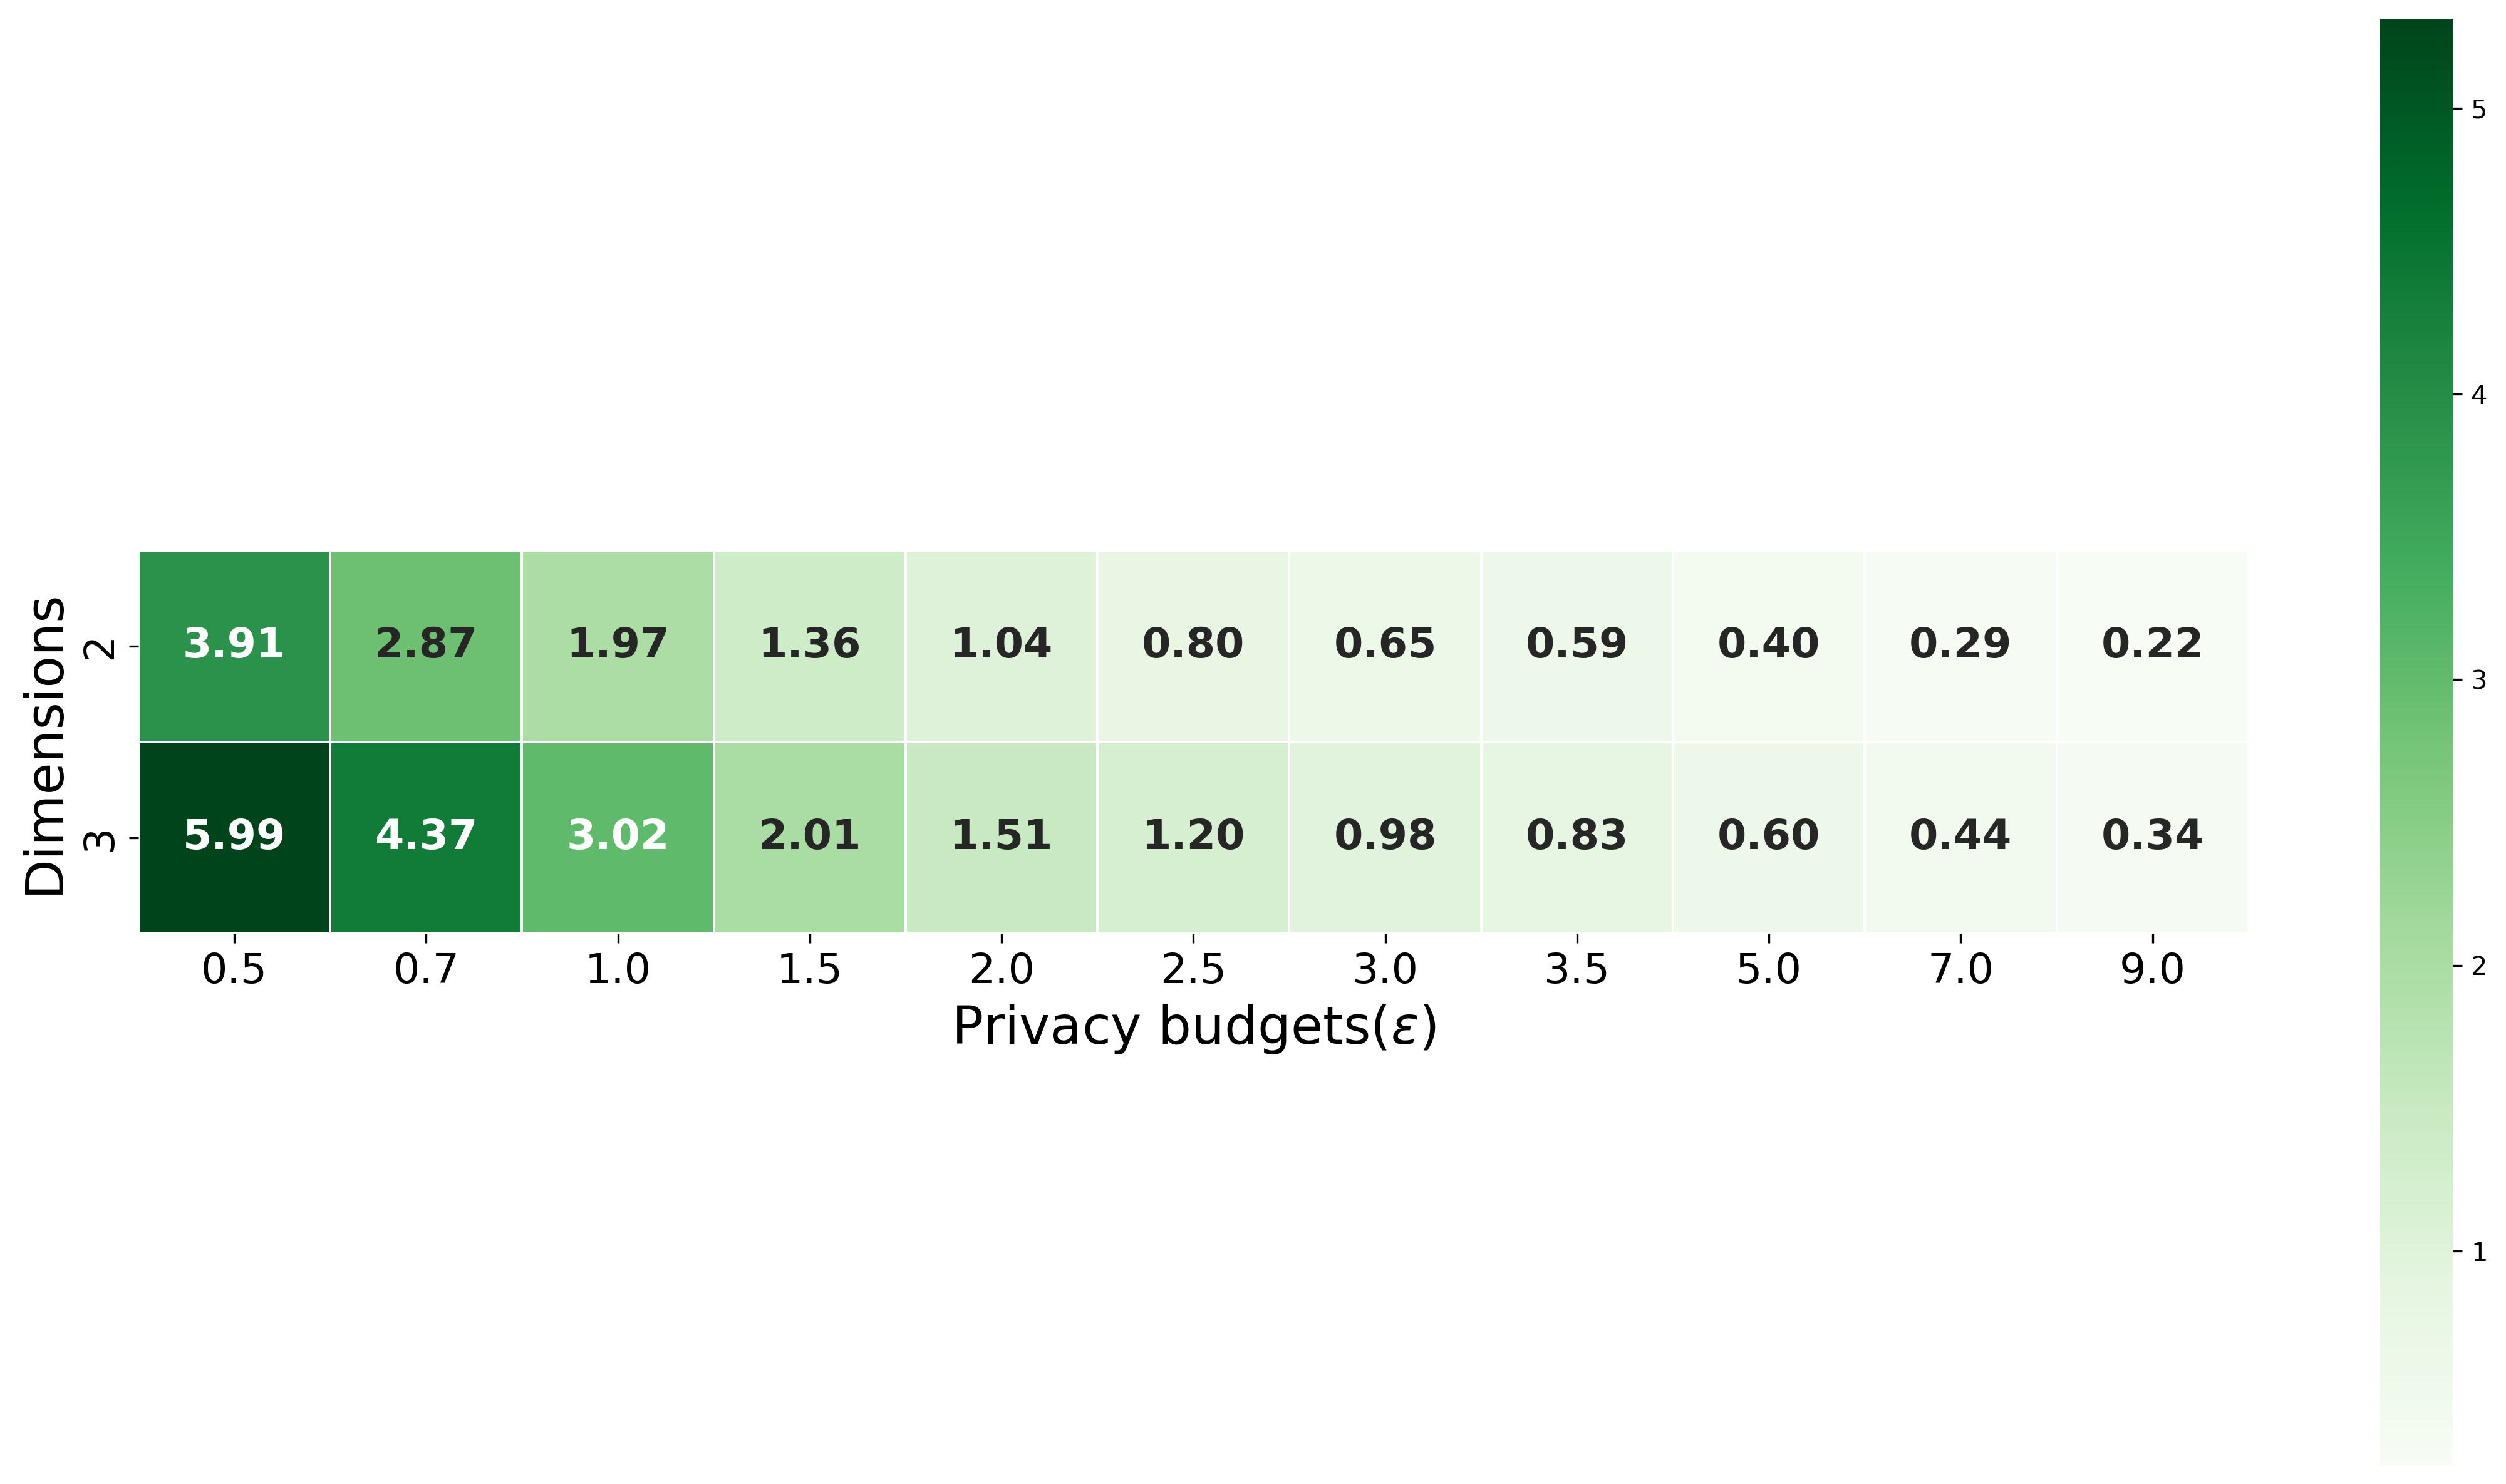
\includegraphics[width=1\textwidth]{Results/kd-laplace/kd-Laplace/skewed-dataset/distance.png}
            \label{fig:privacy-risk_skewed-dataset_adversial_advantage_kd-laplace}
        \end{subfigure}
        \vfill % vertical space

        \begin{subfigure}[c]{1\textwidth}
            \caption{\textbf{Heatmap showing disclosure risk for the Piecewise mechanism, per privacy budget \& dimension for skewed-dataset.}}
            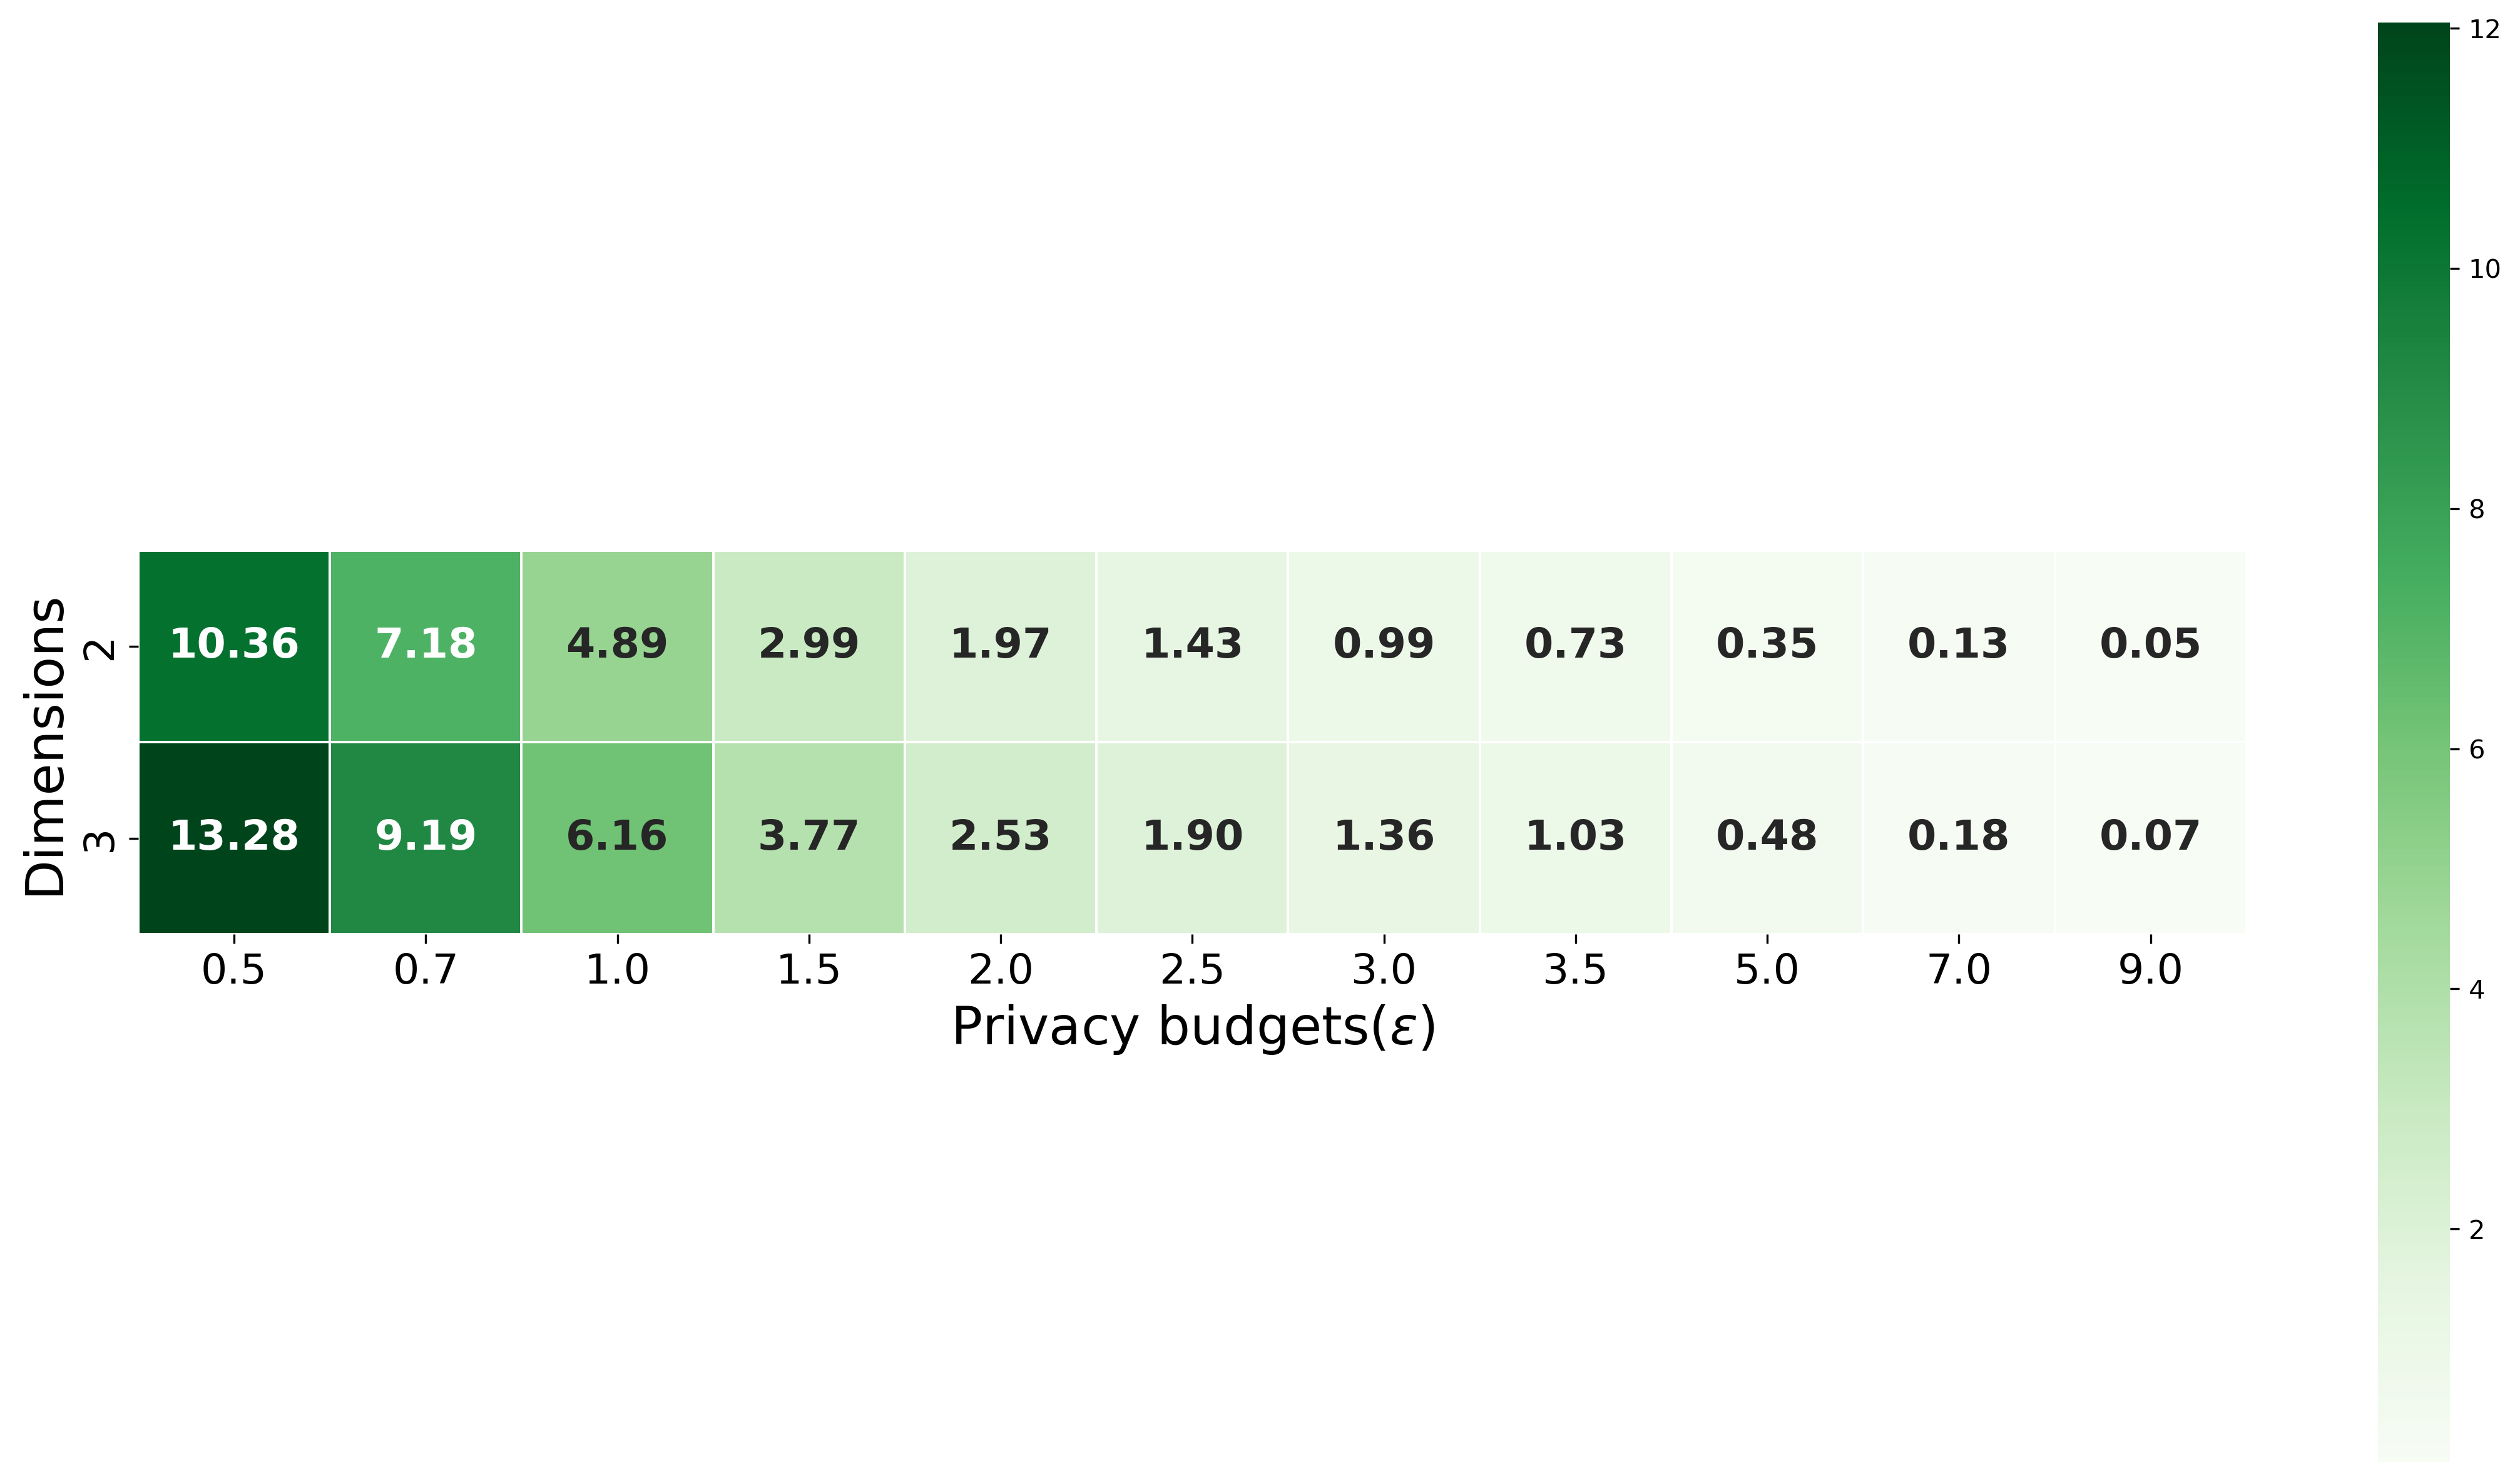
\includegraphics[width=1\textwidth]{Results/kd-laplace/piecewise/skewed-dataset/distance.png}
            \label{fig:privacy-risk_skewed-dataset_adversial_advantage_piecewise}
        \end{subfigure}
    \end{subfigure}
    \hfill % horizontal space
    \begin{subfigure}[b]{0.075\textwidth}
        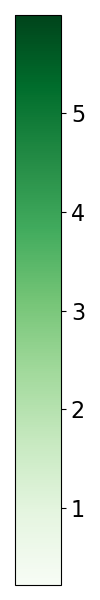
\includegraphics[width=1\textwidth]{Results/kd-laplace/kd-Laplace/skewed-dataset/heatmap_legend_distance.png}
    \end{subfigure}
\end{figure}
\newpage
\begin{figure}[H]
    \centering
    \begin{subfigure}[b]{0.9\textwidth}
        \begin{subfigure}[c]{1\textwidth}
            \caption{\textbf{Heatmap TPR for the kD-Laplace mechanism, per privacy budget \& dimension for skewed-dataset.}}
            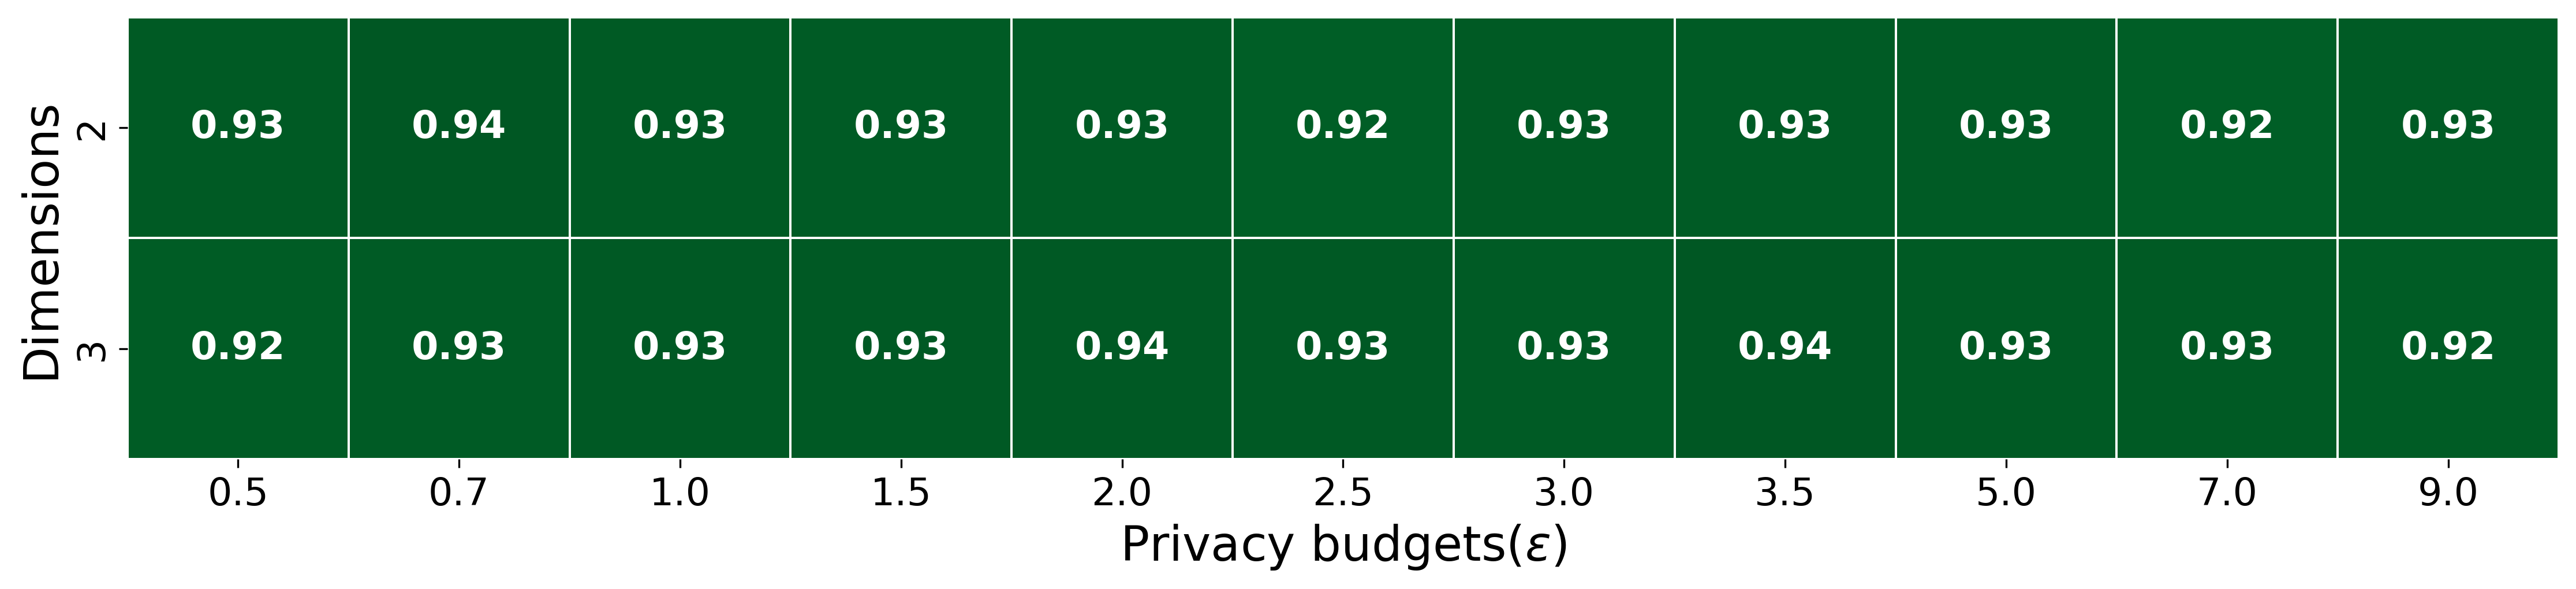
\includegraphics[width=1\textwidth]{Results/kd-laplace/kd-Laplace/skewed-dataset/tpr.png}
            \label{fig:privacy_tpr_skewed-dataset_adversial_advantage_kd-laplace}
        \end{subfigure}
        \vfill % vertical space

        \begin{subfigure}[c]{1\textwidth}
            \caption{\textbf{Heatmap TPR for the Piecewise mechanism, per privacy budget \& dimension for skewed-dataset.}}
            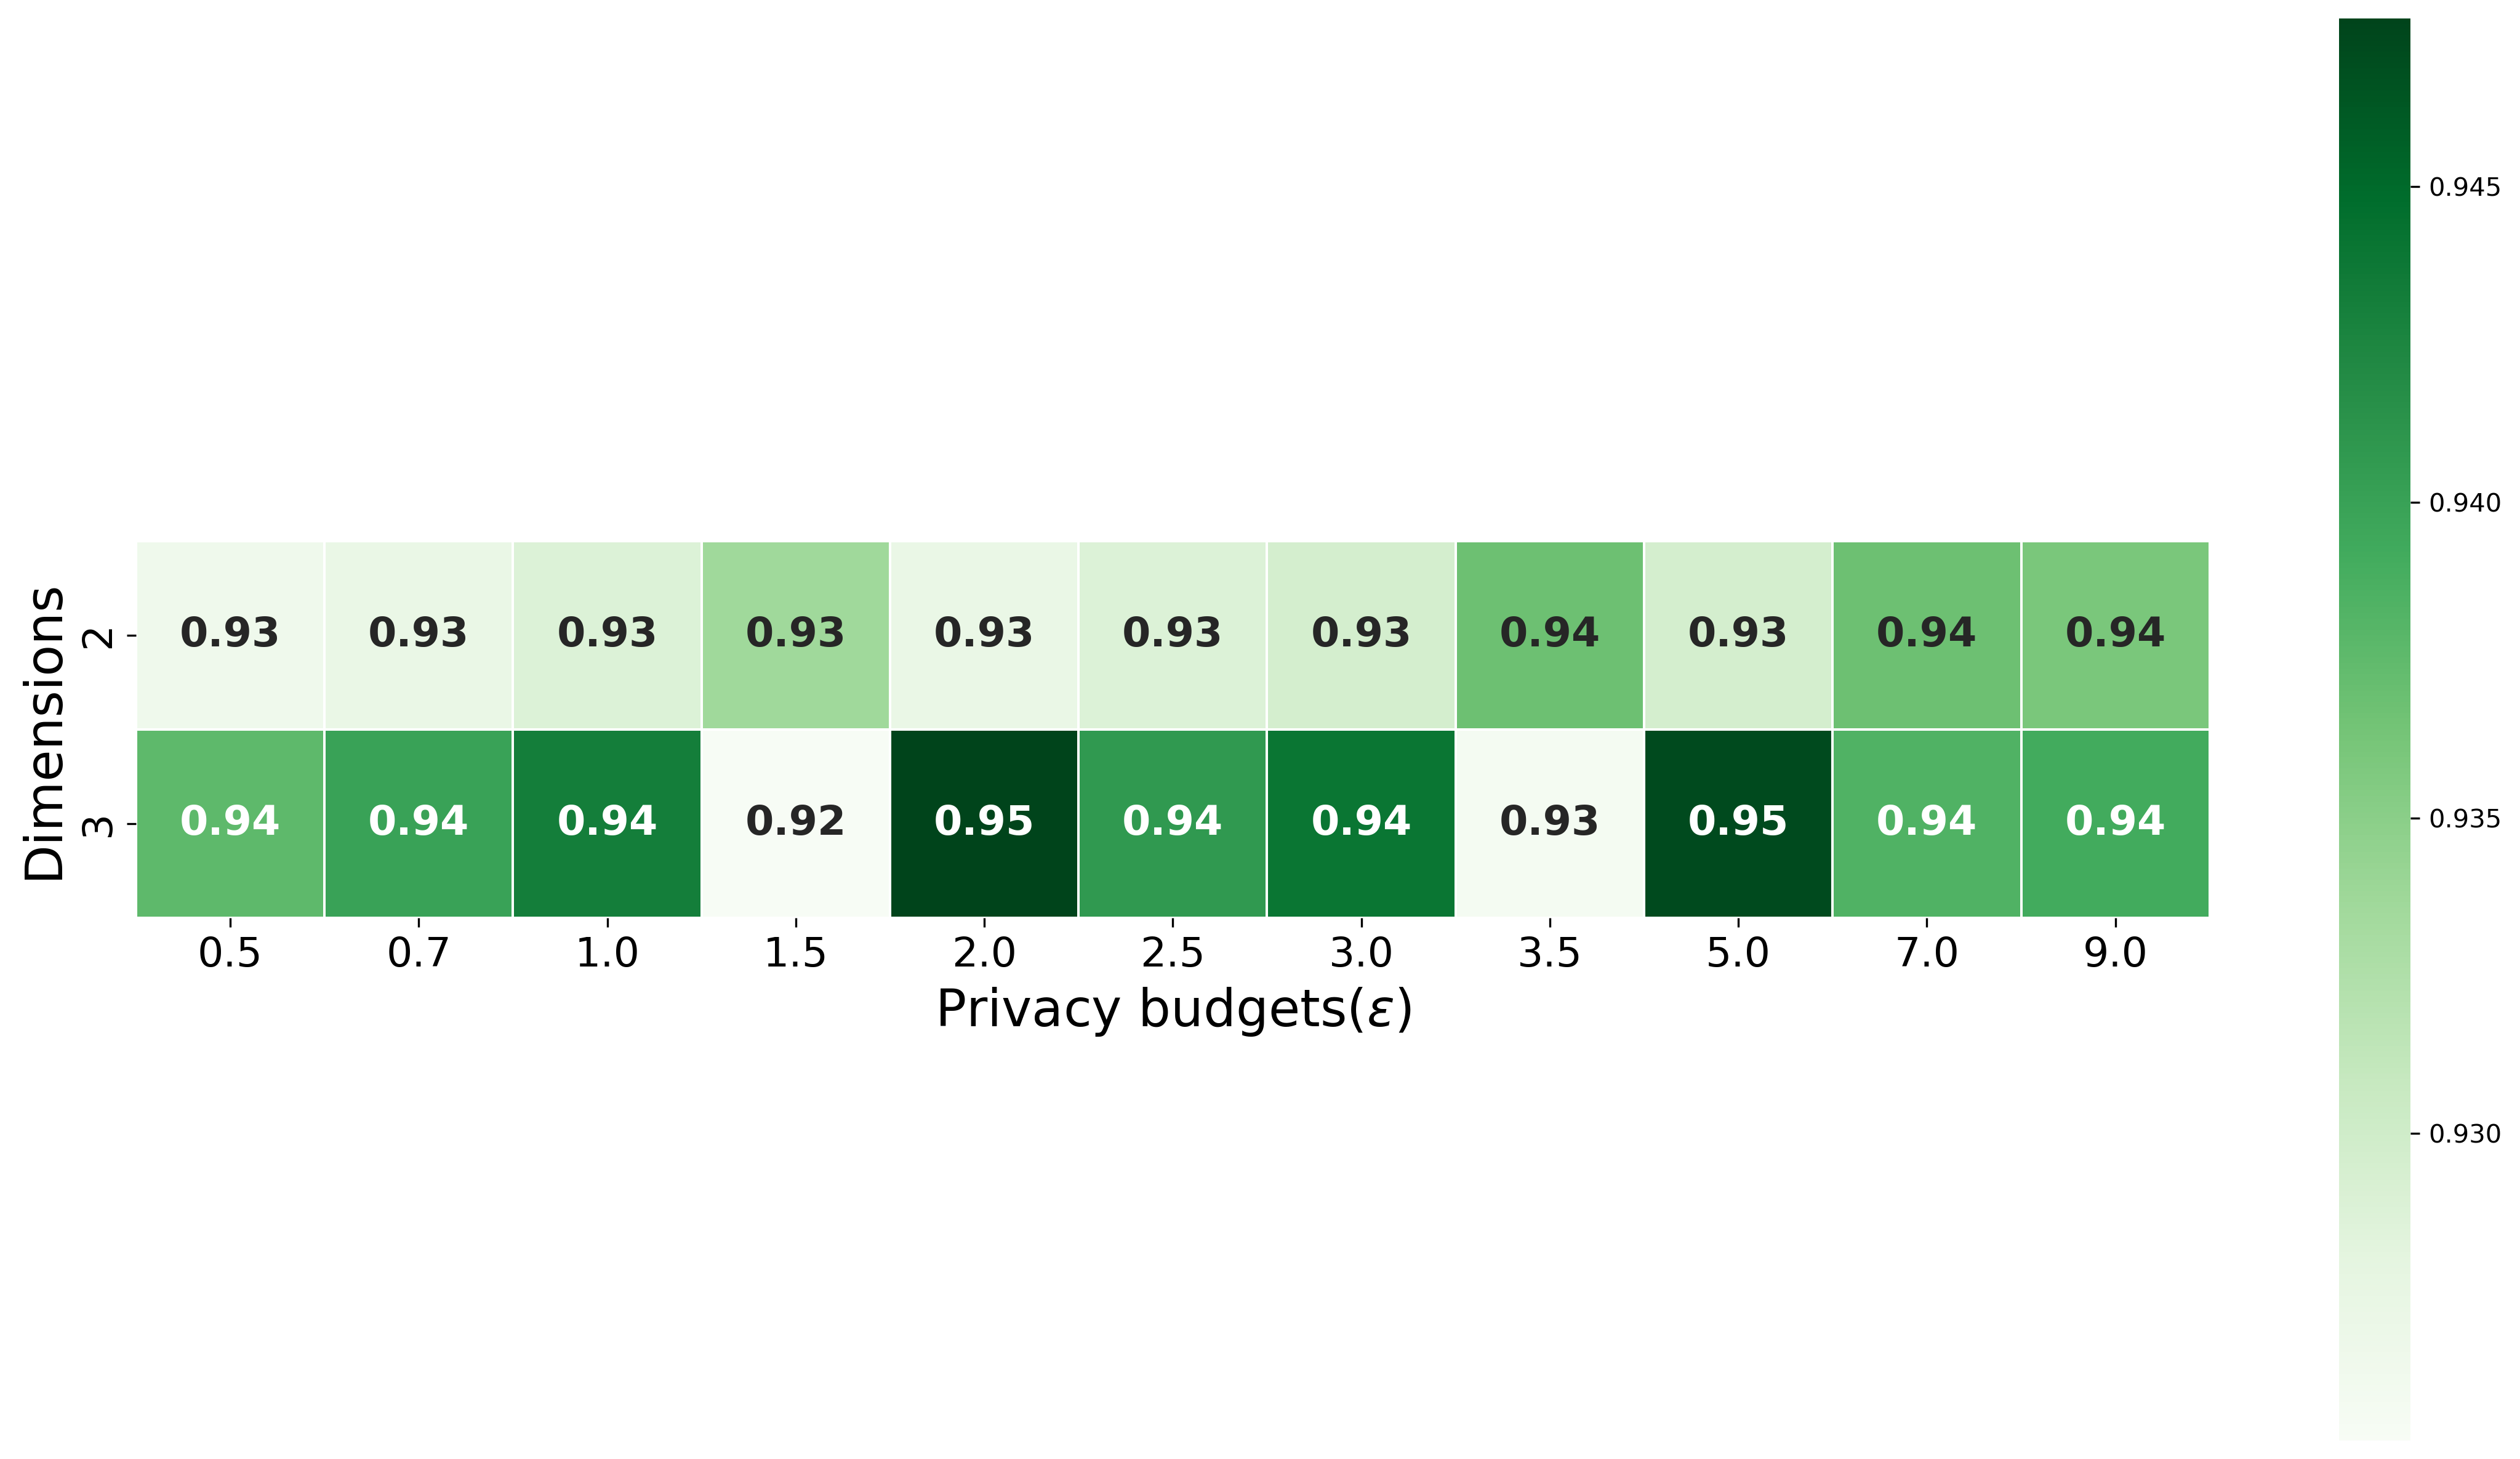
\includegraphics[width=1\textwidth]{Results/kd-laplace/piecewise/skewed-dataset/tpr.png}
            \label{fig:privacy_tpr_skewed-dataset_adversial_advantage_piecewise}
        \end{subfigure}
    \end{subfigure}
    \hfill % horizontal space
    \begin{subfigure}[b]{0.075\textwidth}
        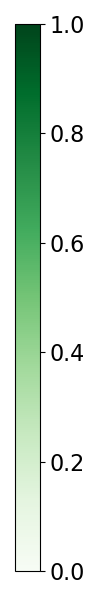
\includegraphics[width=1\textwidth]{Results/kd-laplace/kd-laplace/skewed-dataset/heatmap_legend_tpr.png}
    \end{subfigure}
\end{figure}
\todo[inline]{Add comments}